\documentclass[version=preprint]{iacrcc}
\license{CC-by}

\usepackage{tikz}
\usetikzlibrary{calc,positioning,arrows.meta,shapes.geometric,backgrounds}
%%%%%%%%%%%%%%%%%%%%%%%%%%%%%%%%%%%%%%%%%%%%%%%%%%%%%%%%%%%%%%%%%%%%%%%%%%%%%%%%
%%% TIKZLIBRARY CIPHER %%%%%%%%%%%%%%%%%%%%%%%%%%%%%%%%%%%%%%%%%%%%%%%%%%%%%%%%%
%   Utilities for drawing cryptographic circuits                               %
%   Version: 2024-04-24                                                        %
%   Author: Maria Eichlseder                                                   %
%   \usetikzlibrary{cipher}                                                    %
%%%%%%%%%%%%%%%%%%%%%%%%%%%%%%%%%%%%%%%%%%%%%%%%%%%%%%%%%%%%%%%%%%%%%%%%%%%%%%%%


\makeatletter

%%%%%%%%%%%%%%%%%%%%%%%%%%%%%%%%%%%%%%%%%%%%%%%%%%%%%%%%%%%%%%%%%%%%%%%%%%%%%%%%
%%% SHAPES %%%%%%%%%%%%%%%%%%%%%%%%%%%%%%%%%%%%%%%%%%%%%%%%%%%%%%%%%%%%%%%%%%%%%
%%%%%%%%%%%%%%%%%%%%%%%%%%%%%%%%%%%%%%%%%%%%%%%%%%%%%%%%%%%%%%%%%%%%%%%%%%%%%%%%

%%% UTILS %%%%%%%%%%%%%%%%%%%%%%%%%%%%%%%%%%%%%%%%%%%%%%%%%%%%%%%%%%%%%%%%%%%%%%

% from https://tex.stackexchange.com/questions/14769/add-more-anchors-to-standard-tikz-nodes
\newcommand{\anchorlet}[2]{%
  \global\expandafter
  \let\csname pgf@anchor@\pgf@sm@shape@name @#1\expandafter\endcsname
  \csname pgf@anchor@\pgf@sm@shape@name @#2\endcsname
}

%%% OPERATION SHAPES %%%%%%%%%%%%%%%%%%%%%%%%%%%%%%%%%%%%%%%%%%%%%%%%%%%%%%%%%%%
\pgfdeclareshape{oplus}{%{{{
  \inheritsavedanchors[from=circle]
  \inheritanchorborder[from=circle]
  \foreach \s in {center,mid,base,text, north,south,west,east,
                  mid west,mid east,base west,base east,
                  north west,south west,north east,south east} {
    \inheritanchor[from=circle]{\s}
  }
  %\inheritbackgroundpath[from=circle]
  % From /usr/share/texlive/texmf-dist/tex/generic/pgf/modules/pgfmoduleshapes.code.tex:1148
  \backgroundpath{%
    \pgfutil@tempdima=\radius%
    \pgfmathsetlength{\pgf@xb}{\pgfkeysvalueof{/pgf/outer xsep}}%
    \pgfmathsetlength{\pgf@yb}{\pgfkeysvalueof{/pgf/outer ysep}}%
    \ifdim\pgf@xb<\pgf@yb%
      \advance\pgfutil@tempdima by-\pgf@yb%
    \else%
      \advance\pgfutil@tempdima by-\pgf@xb%
    \fi%
    \pgfpathcircle{\centerpoint}{\pgfutil@tempdima}%
    % north-south
    \centerpoint\advance\pgf@y by\radius  \pgf@xa=\pgf@x \pgf@ya=\pgf@y
    \centerpoint\advance\pgf@y by-\radius \pgf@xb=\pgf@x \pgf@yb=\pgf@y
    \pgfpathmoveto{\pgfpoint{\pgf@xa}{\pgf@ya}}
    \pgfpathlineto{\pgfpoint{\pgf@xb}{\pgf@yb}}
    % east-west
    \centerpoint\advance\pgf@x by\radius  \pgf@xa=\pgf@x \pgf@ya=\pgf@y
    \centerpoint\advance\pgf@x by-\radius \pgf@xb=\pgf@x \pgf@yb=\pgf@y
    \pgfpathmoveto{\pgfpoint{\pgf@xa}{\pgf@ya}}
    \pgfpathlineto{\pgfpoint{\pgf@xb}{\pgf@yb}}
  }
}%}}}

\pgfdeclareshape{ominus}{%{{{
  \inheritsavedanchors[from=circle]
  \inheritanchorborder[from=circle]
  \foreach \s in {center,mid,base,text, north,south,west,east,
                  mid west,mid east,base west,base east,
                  north west,south west,north east,south east} {
    \inheritanchor[from=circle]{\s}
  }
  %\inheritbackgroundpath[from=circle]
  % From /usr/share/texlive/texmf-dist/tex/generic/pgf/modules/pgfmoduleshapes.code.tex:1148
  \backgroundpath{%
    \pgfutil@tempdima=\radius%
    \pgfmathsetlength{\pgf@xb}{\pgfkeysvalueof{/pgf/outer xsep}}%
    \pgfmathsetlength{\pgf@yb}{\pgfkeysvalueof{/pgf/outer ysep}}%
    \ifdim\pgf@xb<\pgf@yb%
      \advance\pgfutil@tempdima by-\pgf@yb%
    \else%
      \advance\pgfutil@tempdima by-\pgf@xb%
    \fi%
    \pgfpathcircle{\centerpoint}{\pgfutil@tempdima}%
    % east-west
    \centerpoint\advance\pgf@x by\radius  \pgf@xa=\pgf@x \pgf@ya=\pgf@y
    \centerpoint\advance\pgf@x by-\radius \pgf@xb=\pgf@x \pgf@yb=\pgf@y
    \pgfpathmoveto{\pgfpoint{\pgf@xa}{\pgf@ya}}
    \pgfpathlineto{\pgfpoint{\pgf@xb}{\pgf@yb}}
  }
}%}}}

\pgfdeclareshape{otimes}{%{{{
  \inheritsavedanchors[from=circle]
  \inheritanchorborder[from=circle]
  \foreach \s in {center,mid,base,text, north,south,west,east,
                  mid west,mid east,base west,base east,
                  north west,south west,north east,south east} {
    \inheritanchor[from=circle]{\s}
  }
  %\inheritbackgroundpath[from=circle]
  % From /usr/share/texlive/texmf-dist/tex/generic/pgf/modules/pgfmoduleshapes.code.tex:1148
  \backgroundpath{%
    \pgfutil@tempdima=\radius%
    \pgfmathsetlength{\pgf@xb}{\pgfkeysvalueof{/pgf/outer xsep}}%
    \pgfmathsetlength{\pgf@yb}{\pgfkeysvalueof{/pgf/outer ysep}}%
    \ifdim\pgf@xb<\pgf@yb%
      \advance\pgfutil@tempdima by-\pgf@yb%
    \else%
      \advance\pgfutil@tempdima by-\pgf@xb%
    \fi%
    \pgfpathcircle{\centerpoint}{\pgfutil@tempdima}%
    % nw-se
    \centerpoint
    \pgf@xc=\radius
    \advance\pgf@x by-0.707107\pgf@xc  \pgf@xa=\pgf@x
    \advance\pgf@y by 0.707107\pgf@xc  \pgf@ya=\pgf@y
    \centerpoint
    \advance\pgf@x by 0.707107\pgf@xc  \pgf@xb=\pgf@x
    \advance\pgf@y by-0.707107\pgf@xc  \pgf@yb=\pgf@y
    \pgfpathmoveto{\pgfpoint{\pgf@xa}{\pgf@ya}}
    \pgfpathlineto{\pgfpoint{\pgf@xb}{\pgf@yb}}
    % sw-ne
    \centerpoint
    \advance\pgf@x by-0.707107\pgf@xc  \pgf@xa=\pgf@x
    \advance\pgf@y by-0.707107\pgf@xc  \pgf@ya=\pgf@y
    \centerpoint
    \advance\pgf@x by 0.707107\pgf@xc  \pgf@xb=\pgf@x
    \advance\pgf@y by 0.707107\pgf@xc  \pgf@yb=\pgf@y
    \pgfpathmoveto{\pgfpoint{\pgf@xa}{\pgf@ya}}
    \pgfpathlineto{\pgfpoint{\pgf@xb}{\pgf@yb}}
  }
}%}}}

\pgfdeclareshape{boxplus}{%{{{
  \inheritsavedanchors[from=rectangle]
  \inheritanchorborder[from=rectangle]
  \foreach \s in {center,mid,base,text, north,south,west,east,
                  mid west,mid east,base west,base east,
                  north west,south west,north east,south east} {
    \inheritanchor[from=rectangle]{\s}
  }
  \backgroundpath{
    % store lower right in xa/ya and upper right in xb/yb
    \southwest \pgf@xa=\pgf@x \pgf@ya=\pgf@y
    \northeast \pgf@xb=\pgf@x \pgf@yb=\pgf@y
    % store center in xc/yc
    \pgf@xc=.5\pgf@xa \advance\pgf@xc by .5\pgf@xb
    \pgf@yc=.5\pgf@ya \advance\pgf@yc by .5\pgf@yb
    % construct main path
    \pgfpathmoveto{\pgfpoint{\pgf@xa}{\pgf@ya}}
    \pgfpathlineto{\pgfpoint{\pgf@xa}{\pgf@yb}}
    \pgfpathlineto{\pgfpoint{\pgf@xb}{\pgf@yb}}
    \pgfpathlineto{\pgfpoint{\pgf@xb}{\pgf@ya}}
    \pgfpathclose
    \pgfpathmoveto{\pgfpoint{\pgf@xc}{\pgf@ya}}
    \pgfpathlineto{\pgfpoint{\pgf@xc}{\pgf@yb}}
    \pgfpathmoveto{\pgfpoint{\pgf@xa}{\pgf@yc}}
    \pgfpathlineto{\pgfpoint{\pgf@xb}{\pgf@yc}}
  }
}%}}}

%%% PRIMITIVE SHAPES %%%%%%%%%%%%%%%%%%%%%%%%%%%%%%%%%%%%%%%%%%%%%%%%%%%%%%%%%%%
\pgfdeclareshape{compressionf}{%{{{
  \inheritsavedanchors[from=rectangle]
  \inheritanchorborder[from=rectangle]

  \foreach \s in {center,base,text,
                  north,south,west,east,
                  north west, south west, north east, south east} {
    \inheritanchor[from=rectangle]{\s}
  }
  \anchor{msg}{\southwest \pgf@xa=\pgf@x
               \northeast \pgf@x=\pgf@xa}
  \anchor{tip}{\southwest \pgf@xa=\pgf@x
               \northeast
               \pgf@x=\pgf@xa
               \advance\pgf@y by \pgf@y}
  \anchor{top}{\southwest \pgf@xa=\pgf@x
               \northeast
               \advance\pgf@x by-.5\pgf@x
               \advance\pgf@x by .5\pgf@xa
               \advance\pgf@y by .5\pgf@y}
  \backgroundpath{
    % store lower right in xa/ya and upper right in xb/yb
    \southwest \pgf@xa=\pgf@x \pgf@ya=\pgf@y
    \northeast \pgf@xb=\pgf@x \pgf@yb=\pgf@y
    \pgf@xc=\pgf@xa
    \pgf@yc=\pgf@yb \advance\pgf@yc by \pgf@yb

    \pgfpathmoveto{\pgfpoint{\pgf@xa}{\pgf@ya}}
    \pgfpathlineto{\pgfpoint{\pgf@xa}{\pgf@yc}}
    \pgfpathlineto{\pgfpoint{\pgf@xb}{\pgf@yb}}
    \pgfpathlineto{\pgfpoint{\pgf@xb}{\pgf@ya}}
    \pgfpathclose
  }
}%}}}

\pgfdeclareshape{compression}{%{{{
  \inheritsavedanchors[from=rectangle]
  \inheritanchorborder[from=rectangle]

  \foreach \s in {center,base,text,
    north,south,west,east,
    north west, south west, north east, south east} {
    \inheritanchor[from=rectangle]{\s}
  }
  \backgroundpath{
    % store lower left in xa/ya and upper right in xb/yb
    \southwest \pgf@xa=\pgf@x \pgf@ya=\pgf@y
    \northeast \pgf@xb=\pgf@x \pgf@yb=\pgf@y
    \pgf@xc=\pgf@xa \advance\pgf@xc by .75\pgf@xa
    \pgf@yc=\pgf@xb \advance\pgf@yc by-.75\pgf@xa

    \pgfpathmoveto{\pgfpoint{\pgf@xa}{\pgf@ya}}
    \pgfpathlineto{\pgfpoint{\pgf@xc}{\pgf@yb}}
    \pgfpathlineto{\pgfpoint{\pgf@yc}{\pgf@yb}}
    \pgfpathlineto{\pgfpoint{\pgf@xb}{\pgf@ya}}
    \pgfpathclose
  }
}%}}}

\pgfdeclareshape{filter}{%{{{
  \inheritsavedanchors[from=rectangle]
  \inheritanchorborder[from=rectangle]

  \foreach \s in {center,base,text,
                  north,south,west,east,
                  north west, south west, north east, south east} {
    \inheritanchor[from=rectangle]{\s}
  }
  \backgroundpath{
    % store lower left in xa/ya and upper right in xb/yb
    \southwest \pgf@xa=\pgf@x \pgf@ya=\pgf@y
    \northeast \pgf@xb=\pgf@x \pgf@yb=\pgf@y
    \pgf@xc=\pgf@xa \advance\pgf@xc by .75\pgf@xa
    \pgf@yc=\pgf@xb \advance\pgf@yc by-.75\pgf@xa

    \pgfpathmoveto{\pgfpoint{\pgf@xa}{\pgf@ya}}
    \pgfpathlineto{\pgfpoint{\pgf@xc}{\pgf@yb}}
    \pgfpathlineto{\pgfpoint{\pgf@yc}{\pgf@yb}}
    \pgfpathlineto{\pgfpoint{\pgf@xb}{\pgf@ya}}
    \pgfpathclose
  }
}%}}}

\pgfdeclareshape{authentication}{%{{{
  \inheritsavedanchors[from=rectangle]
  \inheritanchorborder[from=rectangle]

  \foreach \s in {center,base,text,
                  north,south,west,east,
                  north west, south west, north east, south east} {
    \inheritanchor[from=rectangle]{\s}
  }
  \anchor{tag}{\northeast \pgf@xa=\pgf@x \pgf@ya=\pgf@y
               %\southwest \pgf@x=\pgf@xa}
               \southwest \pgf@x=\pgf@xa \advance\pgf@y by .5\pgf@y \advance\pgf@y by -.5\pgf@ya}
  \anchor{tip}{\northeast \pgf@xa=\pgf@x \pgf@ya=\pgf@y
               \southwest
               \pgf@x=\pgf@xa
               %\advance\pgf@y by \pgf@y}
               \advance\pgf@y by \pgf@y \advance\pgf@y by -\pgf@ya}
  \anchor{bot}{\northeast \pgf@xa=\pgf@x \pgf@ya=\pgf@y
               \southwest
               \advance\pgf@x by-.5\pgf@x
               \advance\pgf@x by .5\pgf@xa
               %\advance\pgf@y by .5\pgf@y}
               \advance\pgf@y by .5\pgf@y \advance\pgf@y by -.5\pgf@ya}
  \backgroundpath{
    % store upper right in xa/ya and lower left in xb/yb
    \northeast \pgf@xa=\pgf@x \pgf@ya=\pgf@y
    \southwest \pgf@xb=\pgf@x \pgf@yb=\pgf@y
    \pgf@xc=\pgf@xa
    %\pgf@yc=\pgf@yb \advance\pgf@yc by \pgf@yb
    \pgf@yc=\pgf@yb \advance\pgf@yc by \pgf@yb \advance\pgf@yc by -\pgf@ya

    \pgfpathmoveto{\pgfpoint{\pgf@xa}{\pgf@ya}}
    \pgfpathlineto{\pgfpoint{\pgf@xa}{\pgf@yc}}
    \pgfpathlineto{\pgfpoint{\pgf@xb}{\pgf@yb}}
    \pgfpathlineto{\pgfpoint{\pgf@xb}{\pgf@ya}}
    \pgfpathclose
  }
}%}}}

\pgfdeclareshape{wide}{%{{{
  \inheritsavedanchors[from=rectangle]
  \inheritanchorborder[from=rectangle]

  \foreach \s in {center,base,text,
                  north,south,west,east,
                  north west, south west, north east, south east} {
    \inheritanchor[from=rectangle]{\s}
  }
  \anchor{wnw}{\northeast \pgf@xa=\pgf@x \pgf@ya=\pgf@y
               \southwest \advance\pgf@y by-.75\pgf@y
                          \advance\pgf@y by .75\pgf@ya}
  \anchor{wsw}{\northeast \pgf@xa=\pgf@x \pgf@ya=\pgf@y
               \southwest \advance\pgf@y by-.25\pgf@y
                          \advance\pgf@y by .25\pgf@ya}
  \anchor{ene}{\southwest \pgf@xa=\pgf@x \pgf@ya=\pgf@y
               \northeast \advance\pgf@y by-.25\pgf@y
                          \advance\pgf@y by .25\pgf@ya}
  \anchor{ese}{\southwest \pgf@xa=\pgf@x \pgf@ya=\pgf@y
               \northeast \advance\pgf@y by-.75\pgf@y
                          \advance\pgf@y by .75\pgf@ya}

  \anchor{nnw}{\southwest \pgf@xa=\pgf@x \pgf@ya=\pgf@y
               \northeast \advance\pgf@x by-.75\pgf@x
                          \advance\pgf@x by .75\pgf@xa}
  \anchor{nne}{\southwest \pgf@xa=\pgf@x \pgf@ya=\pgf@y
               \northeast \advance\pgf@x by-.25\pgf@x
                          \advance\pgf@x by .25\pgf@xa}
  \anchor{ssw}{\northeast \pgf@xa=\pgf@x \pgf@ya=\pgf@y
               \southwest \advance\pgf@x by-.25\pgf@x
                          \advance\pgf@x by .25\pgf@xa}
  \anchor{sse}{\northeast \pgf@xa=\pgf@x \pgf@ya=\pgf@y
               \southwest \advance\pgf@x by-.75\pgf@x
                          \advance\pgf@x by .75\pgf@xa}

  \inheritbackgroundpath[from=rectangle]

  \anchorlet{xouter}{wnw}
  \anchorlet{youter}{ene}
  \anchorlet{xinner}{wsw}
  \anchorlet{yinner}{ese}
}%}}}

% TODO keyed north/west/south/east

%%% OTHER SHAPES %%%%%%%%%%%%%%%%%%%%%%%%%%%%%%%%%%%%%%%%%%%%%%%%%%%%%%%%%%%%%%%
\pgfdeclareshape{document}{%{{{
  % paper with folded corner
  % from PGF manual, "Command for Declare New Shapes"
  \inheritsavedanchors[from=rectangle]
  \inheritanchorborder[from=rectangle]
  %\inheritanchor[from=rectangle]{center}
  %\inheritanchor[from=rectangle]{north}
  %\inheritanchor[from=rectangle]{south}
  %\inheritanchor[from=rectangle]{west}
  %\inheritanchor[from=rectangle]{east}
  \foreach \s in {center,mid,base,text,north,south,west,east,
                  mid west,mid east,base west,base east,
                  north west,south west,north east,south east} {
    \inheritanchor[from=rectangle]{\s}
  }
  \backgroundpath{
    % store lower right in xa/ya and upper right in xb/yb
    \southwest \pgf@xa=\pgf@x \pgf@ya=\pgf@y
    \northeast \pgf@xb=\pgf@x \pgf@yb=\pgf@y
    % compute corner of ‘‘flipped page’’
    \pgf@xc=\pgf@xb \advance\pgf@xc by-5pt % this should be a parameter
    \pgf@yc=\pgf@yb \advance\pgf@yc by-5pt
    % construct main path
    \pgfpathmoveto{\pgfpoint{\pgf@xa}{\pgf@ya}}
    \pgfpathlineto{\pgfpoint{\pgf@xa}{\pgf@yb}}
    \pgfpathlineto{\pgfpoint{\pgf@xc}{\pgf@yb}}
    \pgfpathlineto{\pgfpoint{\pgf@xb}{\pgf@yc}}
    \pgfpathlineto{\pgfpoint{\pgf@xb}{\pgf@ya}}
    \pgfpathclose
    % add little corner
    \pgfpathmoveto{\pgfpoint{\pgf@xc}{\pgf@yb}}
    \pgfpathlineto{\pgfpoint{\pgf@xc}{\pgf@yc}}
    \pgfpathlineto{\pgfpoint{\pgf@xb}{\pgf@yc}}
    \pgfpathlineto{\pgfpoint{\pgf@xc}{\pgf@yc}}
  }
}
\pgfdeclareshape{minidocument}{
  % paper with folded corner
  % from PGF manual, "Command for Declare New Shapes"
  \inheritsavedanchors[from=rectangle]
  \inheritanchorborder[from=rectangle]
  \inheritanchor[from=rectangle]{center}
  \inheritanchor[from=rectangle]{north}
  \inheritanchor[from=rectangle]{south}
  \inheritanchor[from=rectangle]{west}
  \inheritanchor[from=rectangle]{east}
  \backgroundpath{
    % store lower right in xa/ya and upper right in xb/yb
    \southwest \pgf@xa=\pgf@x \pgf@ya=\pgf@y
    \northeast \pgf@xb=\pgf@x \pgf@yb=\pgf@y
    % compute corner of ‘‘flipped page’’
    \pgf@xc=\pgf@xb \advance\pgf@xc by-2pt % this should be a parameter
    \pgf@yc=\pgf@yb \advance\pgf@yc by-2pt
    % construct main path
    \pgfpathmoveto{\pgfpoint{\pgf@xa}{\pgf@ya}}
    \pgfpathlineto{\pgfpoint{\pgf@xa}{\pgf@yb}}
    \pgfpathlineto{\pgfpoint{\pgf@xc}{\pgf@yb}}
    \pgfpathlineto{\pgfpoint{\pgf@xb}{\pgf@yc}}
    \pgfpathlineto{\pgfpoint{\pgf@xb}{\pgf@ya}}
    \pgfpathclose
    % add little corner
    \pgfpathmoveto{\pgfpoint{\pgf@xc}{\pgf@yb}}
    \pgfpathlineto{\pgfpoint{\pgf@xc}{\pgf@yc}}
    \pgfpathlineto{\pgfpoint{\pgf@xb}{\pgf@yc}}
    \pgfpathlineto{\pgfpoint{\pgf@xc}{\pgf@yc}}
  }
}
\tikzset{doc/.style={draw, fill=none, shape=document}}
\tikzset{minidoc/.style={draw, fill=none, shape=minidocument}}
%}}}

%%%%%%%%%%%%%%%%%%%%%%%%%%%%%%%%%%%%%%%%%%%%%%%%%%%%%%%%%%%%%%%%%%%%%%%%%%%%%%%%
%%% MATRIX STATE %%%%%%%%%%%%%%%%%%%%%%%%%%%%%%%%%%%%%%%%%%%%%%%%%%%%%%%%%%%%%%%
%%%%%%%%%%%%%%%%%%%%%%%%%%%%%%%%%%%%%%%%%%%%%%%%%%%%%%%%%%%%%%%%%%%%%%%%%%%%%%%%
\providecommand{\State}[1]{\MatrixState{#1}}  % load library late to avoid name conflicts
\newcommand{\MatrixState}[1]{%
  \tikz[stateopts]{
    \foreach \x/\y/\s in {0/0/0, 0/1/1, 0/2/2, 0/3/3,
                          1/0/4, 1/1/5, 1/2/6, 1/3/7,
                          2/0/8, 2/1/9, 2/2/10,2/3/11,
                          3/0/12,3/1/13,3/2/14,3/3/15} {
       %
      \draw (\y+.5,-\x-.5) coordinate (s\s) coordinate (ss\x\y); % (rowwise indices)
      \draw (\x+.5,-\y-.5) coordinate (b\s); % AES indices (columnwise)
    }
    \draw (2,-2) coordinate (label);
    #1
    \draw (0,0) rectangle (4,-4);
    \foreach \x in {1,2,3} {
      \draw[raster] (0,-\x) -- ++(4,0);
      \draw[raster] (\x,0) -- ++(0,-4);
    }
  }%
}
\newcommand{\Column}[1]{%
  \tikz[stateopts]{
    \foreach \x/\y/\s in {0/0/0, 1/0/4, 2/0/8, 3/0/12} {
      \draw (\y+.5,-\x-.5) coordinate (s\s) coordinate (ss\x\y); % (rowwise indices)
    }
    #1
    \draw (0,0) rectangle (1,-4);
    \foreach \x in {1,2,3} { \draw[raster] (0,-\x) -- ++(1,0); }
  }%
}

\newcommand{\Cell}[2]{\draw (#1) node[inner sep=0pt,cellopts] {#2\vphantom{0}};}
\newcommand{\FillCell}[2][fillopts]{\fill[#1] (#2) ++(-.5,.5) rectangle +(1,-1);}
\newcommand{\FillCells}[2][fillopts]{\foreach \s in {#2} {\FillCell[#1]{ss\s}}}
\newcommand{\Fill}[2][fillopts]{\FillCell[#1]{#2}}
\newcommand{\FillColumn}[2][fillopts]{\fill[#1] (ss0#2) ++(-.5,.5) rectangle +(1,-4);}
\newcommand{\FillDiagonal}[2][fillopts]{\foreach \dd in {0,...,3} {\pgfmathsetmacro{\dx}{mod(int(\dd)+int(#2),4)}\Fill[#1]{ss\dd\dx}}}
\newcommand{\FillAntiDiagonal}[2][fillopts]{\foreach \dd in {0,...,3} {\pgfmathsetmacro{\dx}{mod(int(#2)+4-int(\dd),4)}\Fill[#1]{ss\dd\dx}}}
\newcommand{\FillState}[1][fillopts]{\fill[#1] (0,0) rectangle (4,-4);}

\newcommand{\TFill}[2][tfillopts]{\fill[#1] (#2) ++(-.5,.5) -- +(0,-1) -- +(1,0) -- cycle;}
\newcommand{\BFill}[2][bfillopts]{\fill[#1] (#2) ++(.5,-.5) -- +(0,1) -- +(-1,0) -- cycle;}
\newcommand{\TFillCells}[2][tfillopts]{\foreach \s in {#2} {\TFill[#1]{ss\s}}}
\newcommand{\BFillCells}[2][bfillopts]{\foreach \s in {#2} {\BFill[#1]{ss\s}}}

% TODO check out if TiKZ matrices (tikzmanual.pdf Chapter 20) could be useful instead

%%%%%%%%%%%%%%%%%%%%%%%%%%%%%%%%%%%%%%%%%%%%%%%%%%%%%%%%%%%%%%%%%%%%%%%%%%%%%%%%
%%% ARROWS %%%%%%%%%%%%%%%%%%%%%%%%%%%%%%%%%%%%%%%%%%%%%%%%%%%%%%%%%%%%%%%%%%%%%
%%%%%%%%%%%%%%%%%%%%%%%%%%%%%%%%%%%%%%%%%%%%%%%%%%%%%%%%%%%%%%%%%%%%%%%%%%%%%%%%
\usetikzlibrary{arrows.meta}
\pgfarrowsdeclare{ipe arrow}{ipe arrow}{%{{{
  \pgfutil@tempdima=5pt\relax
  \advance\pgfutil@tempdima-1.5\pgflinewidth
  \pgfarrowsleftextend{+-\pgfutil@tempdima}%
  \pgfarrowsrightextend{+1.5\pgflinewidth}%
}{%
  \pgftransformshift{\pgfqpoint{1.5\pgflinewidth}{0pt}}%
  \pgfpathmoveto{\pgfpointorigin}%
  \pgfpathlineto{\pgfqpoint{-5pt}{-1.666pt}}%
  \pgfpathlineto{\pgfqpoint{-5pt}{+1.666pt}}%
  \pgfpathclose
  \pgfusepathqfill
}%}}}
\makeatother

%%%%%%%%%%%%%%%%%%%%%%%%%%%%%%%%%%%%%%%%%%%%%%%%%%%%%%%%%%%%%%%%%%%%%%%%%%%%%%%%
%%% STYLES %%%%%%%%%%%%%%%%%%%%%%%%%%%%%%%%%%%%%%%%%%%%%%%%%%%%%%%%%%%%%%%%%%%%%
%%%%%%%%%%%%%%%%%%%%%%%%%%%%%%%%%%%%%%%%%%%%%%%%%%%%%%%%%%%%%%%%%%%%%%%%%%%%%%%%

%%% OPERATION STYLES %%%%%%%%%%%%%%%%%%%%%%%%%%%%%%%%%%%%%%%%%%%%%%%%%%%%%%%%%%%
\tikzset{op/.style={draw, fill=none, minimum size=1.5ex, inner sep=0pt}}
\tikzset{xor/.style={op, shape=oplus}}
\tikzset{not/.style={op, shape=ominus}}
\tikzset{mul/.style={op, shape=otimes}}
\tikzset{and/.style={op, shape=otimes}} % TODO \odot
\tikzset{sum/.style={op, shape=boxplus}}
\tikzset{tee/.style={shape=circle, fill, draw, inner sep=0pt, minimum size=2pt}}
\tikzset{rot/.style={shape=rectangle, draw, inner sep=2pt, rounded corners=2pt}} % TODO

%%% PRIMITIVE STYLES %%%%%%%%%%%%%%%%%%%%%%%%%%%%%%%%%%%%%%%%%%%%%%%%%%%%%%%%%%%
\tikzset{box/.style={minimum size=.75cm, draw, inner sep=1pt, fill=white, rounded corners=3pt}}
\tikzset{oper/.style={box,inner sep=1pt,minimum width=.3cm,font=\scriptsize,align=center}}

\tikzset{
  key west/.style={path picture={\draw[line cap=round,rounded corners=0pt] (path picture bounding box.west) +(.25pt,.65ex) -- +(.65ex,0) -- +(.25pt,-.65ex);}},
  key east/.style={path picture={\draw[line cap=round,rounded corners=0pt] (path picture bounding box.east) +(-.25pt,.65ex) -- +(-.65ex,0) -- +(-.25pt,-.65ex);}},
  key north/.style={path picture={\draw[line cap=round,rounded corners=0pt] (path picture bounding box.north) +(-.65ex,-.25pt) -- +(0,-.65ex) -- +(.65ex,-.25pt);}},
  key south/.style={path picture={\draw[line cap=round,rounded corners=0pt] (path picture bounding box.south) +(-.65ex,.25pt) -- +(0,.65ex) -- +(.65ex,.25pt);}},
  key at/.style args = {#1}{path picture={\draw[line cap=round,rounded corners=0pt] (path picture bounding box.#1) +(-.65ex,.25pt) -- +(0,.65ex) -- +(.65ex,.25pt);}},
}

%%% ARROW STYLES %%%%%%%%%%%%%%%%%%%%%%%%%%%%%%%%%%%%%%%%%%%%%%%%%%%%%%%%%%%%%%%
\tikzset{next/.style={->, >=ipe arrow}}
\tikzset{prev/.style={<-, >=ipe arrow}}

%%% MATRIX STATE %%%%%%%%%%%%%%%%%%%%%%%%%%%%%%%%%%%%%%%%%%%%%%%%%%%%%%%%%%%%%%%
\tikzset{
  state/.style={inner sep=0pt},
  stateopts/.style={scale=.3},
  raster/.style={},
  fillopts/.style={gray},
  tfillopts/.style={gray},
  bfillopts/.style={gray},
  cellopts/.style={},
}

% TODO provide settings that prefill nodes with \State{}

% TODO alternative shapes -- careful, they mess up with chained comments and relative coordinates!
\tikzset{
  notalt/.style={draw,circle,append after command={
                 [shorten >=\pgflinewidth, shorten <=\pgflinewidth]
                 (\tikzlastnode.east) edge (\tikzlastnode.west)
                }},
  xoralt/.style={draw,circle,append after command={
                 [shorten >=\pgflinewidth, shorten <=\pgflinewidth]
                 (\tikzlastnode.north) edge (\tikzlastnode.south)
                 (\tikzlastnode.east) edge (\tikzlastnode.west)
                }},
  andalt/.style={op, shape=circle, every label/.style={}, label={center:\tikz{\filldraw circle (.75pt);}} },
}

\newcommand{\CipherInit}[2]{
  % #1 = label
  % #2 = state
  \coordinate (init);
  \draw (init) coordinate (here); % current x-coordinate of state
  \draw (here)  node[state,label={#1}] (S) {\MatrixState{#2}};
  \draw (S.east) coordinate (Shere);
}

\newcommand{\CipherStep}[3]{
  % #1 = operation
  % #2 = label
  % #3 = state

  \draw (Shere.east) coordinate (Sprev);
  \draw (S) ++(1.8,0) node[state,label={#2}] (S) {\MatrixState{#3}};
  \draw[->] (Sprev) -- node[oper,align=center] {#1} (S);
  \draw (S.east) coordinate (Shere);
}

\newcommand{\CipherAddK}[4]{
  % #1 = label
  % #2 = state
  % #3 = keylabel
  % #4 = keystate

  \draw (Shere.east) coordinate (Sprev);
  \draw (S) ++(5*\stateScale,-\stateScale) node[state,label={#1}] (S) {\MatrixState{#2}};
  \draw (S.north) -- ++(0,.5*\stateScale) coordinate[xor] (Txor);
  \draw[->,rounded corners=1pt] (Sprev) -- +(.5*\stateScale,0) |- (Txor);

  \draw (S) ++(5*\stateScale,+\stateScale) node[state,label={#3}] (S) {\MatrixState{#4}};
  \draw[<-,rounded corners=1pt] (S.west) -- +(-.5*\stateScale,0) |- (Txor);
  \draw (S.east) coordinate (Shere);
}

\newcommand{\CipherLine}[2]{
  \draw (S.east) coordinate (Send) ++(\stateScale,-3.5*\stateScale) coordinate (Shookend);
  \draw (init) +(0,-6*\stateScale) coordinate (init);
  \draw (init)  node[state,label={#1}] (S) {\MatrixState{#2}};
  \draw (S.west) +(-\stateScale,0) coordinate (Shookstart);
  \draw[->,rounded corners=2pt] (Send) -| (Shookend) -| (Shookstart) -- (S.west);
  \draw (S.east) coordinate (Shere);
}

\newcommand{\stateScale}{.3}

% vim: foldmethod=marker

\usepackage{pgfplots}
\pgfplotsset{compat=1.18}
\usepackage{amsmath,amsfonts,amssymb}
\usepackage{graphicx}
\usepackage{booktabs,multirow,array}
\usepackage{subcaption}
\usepackage[ruled,vlined,linesnumbered]{algorithm2e}
\usepackage{xcolor}

\AtBeginDocument{%
  \hypersetup{
    colorlinks=true,
    linkcolor=blue,
    citecolor=blue,
    urlcolor=blue,
  }%
}
\def\tableautorefname{Table}
\def\appendixautorefname{Appendix}
\def\sectionautorefname{Section}
\renewcommand{\sectionautorefname}{Section}
\renewcommand{\tableautorefname}{Table}
\providecommand{\algorithmautorefname}{Algorithm}
\providecommand{\definitionautorefname}{Definition}
\providecommand{\lemmaautorefname}{Lemma}
\providecommand{\theoremautorefname}{Theorem}
\providecommand{\corollaryautorefname}{Corollary}
\providecommand{\propositionautorefname}{Proposition}
\providecommand{\exampleautorefname}{Example}
\providecommand{\remarkautorefname}{Remark}
\providecommand{\NLF}{\mathsf{NLF}}

\title[running = {Revisiting Practical Attacks on KeeLoq}]{Revisiting Practical Attacks on KeeLoq}

\addauthor[orcid   = {0000-0002-3820-3765},
           inst    = {1},
           email   = {hosein.hadipour@rub.de},
           surname = {Hadipour}
          ]{Hosein Hadipour}

\authorrunning{Hosein Hadipour}

\addaffiliation[city = {Bochum},
                country = {Germany}
               ]{Ruhr University Bochum}

\begin{document}

\maketitle

\keywords{KeeLoq, cryptanalysis, GPU, fixed points, slide attacks, meet-in-the-middle}

\begin{abstract}
KeeLoq is a 32-bit block cipher with a 64-bit key that is used in remote controls and other low-cost authentication devices.
Although KeeLoq has been known to admit key-recovery attacks for more than fifteen years, the published attacks have lacked reproducible comparisons on current hardware.
We analyze three established attack settings and refine the earlier full-codebook fixed-point attack, which assumes access to all $2^{32}$ plaintext--ciphertext pairs.
Our main analytical contribution targets plaintexts that return to their initial value after eight applications of KeeLoq's 64-round core.
Under the standard model that treats this core as a random permutation, the resulting attack succeeds with probability $1-e^{-15/8}\approx84.7\%$, compared with about $30\%$ or $63\%$ for earlier attacks under the same full-codebook assumption.
It recovered 85 of 100 experimental keys, with a mean time of 6.2 seconds over successful cases; most of this time was spent solving Boolean satisfiability problems on the CPU.
For practical context, a parallel exhaustive search using two known pairs reaches a median $2^{37.36}$ tested keys per second on an NVIDIA RTX PRO~6000, implying an expected search time of 1.65 years on one GPU.
Finally, we implement the known slide meet-in-the-middle attack, which uses about $2^{16}$ known pairs and succeeds with probability about $63\%$.
A complete scan is estimated to take 5.0 hours from measurements covering 64 of the $2^{16}$ values of one 16-bit key fragment.
This work improves the fixed-point success bound and provides reproducible measurements; it does not claim a new theoretical complexity for the slide attack.
\end{abstract}

\begin{textabstract}
KeeLoq is a 32-bit block cipher with a 64-bit key that is used in remote controls and other low-cost authentication devices.
Although KeeLoq has been known to admit key-recovery attacks for more than fifteen years, the published attacks have lacked reproducible comparisons on current hardware.
We analyze three established attack settings and refine the earlier full-codebook fixed-point attack, which assumes access to all 2^32 plaintext-ciphertext pairs.
Our main analytical contribution targets plaintexts that return to their initial value after eight applications of KeeLoq's 64-round core.
Under the standard model that treats this core as a random permutation, the resulting attack succeeds with probability 1-exp(-15/8), approximately 84.7%, compared with about 30% or 63% for earlier attacks under the same full-codebook assumption.
It recovered 85 of 100 experimental keys, with a mean time of 6.2 seconds over successful cases; most of this time was spent solving Boolean satisfiability problems on the CPU.
For practical context, a parallel exhaustive search using two known pairs reaches a median 2^37.36 tested keys per second on an NVIDIA RTX PRO 6000, implying an expected search time of 1.65 years on one GPU.
Finally, we implement the known slide meet-in-the-middle attack, which uses about 2^16 known pairs and succeeds with probability about 63%.
A complete scan is estimated to take 5.0 hours from measurements covering 64 of the 2^16 values of one 16-bit key fragment.
This work improves the fixed-point success bound and provides reproducible measurements; it does not claim a new theoretical complexity for the slide attack.
\end{textabstract}

\section{Introduction}\label{sec:introduction}

KeeLoq is a lightweight block cipher with a 32-bit block and a 64-bit key.
It has been used in remote keyless entry systems, passive entry systems, immobilizers, garage and gate openers, and related low-cost devices~\cite{bogdanov2007linear,indesteege2008practical}.
Its round function is very small and its key schedule repeats every 64 rounds.
These two properties make the cipher efficient in hardware, but they also create structural weaknesses.

The full cipher uses 528 rounds.
Because the key schedule has period 64, the encryption can be written as
\[
E_{528} = E_{16} \circ F^8,
\]
where $F = E_{64}$ denotes one 64-round segment.
This identity suggests two natural attack directions:
fixed points of $F^8$, and slid pairs for $F$ combined with a meet-in-the-middle key recovery.
Alongside them, exhaustive key search remains the universal baseline.

Earlier work already showed that KeeLoq is vulnerable to several strong attacks:
Bogdanov studied linear slide attacks with full-codebook data~\cite{bogdanov2007linear};
Courtois, Bard, and Wagner studied fixed-point and cycle structure based attacks~\cite{courtois2007algebraic};
and Aerts et al.\ gave a practical slide meet-in-the-middle attack (S/MITM) using about $2^{16}$ known plaintext-ciphertext pairs and time about $2^{44.5}$ full encryptions~\cite{indesteege2008practical}.
Together, these works established the main cryptanalytic picture of KeeLoq.
They also make an important distinction in data access.
The full-codebook setting gives the adversary all $2^{32}$ possible plaintexts and their ciphertexts.
It is useful for understanding structural weakness, but it is usually a very strong assumption for real systems.
By contrast, the $2^{16}$ pair setting is much closer to the challenge response use cases discussed in~\cite{indesteege2008practical}.

What has been missing is a reproducible comparison of these attacks under clearly stated data assumptions, success criteria, and measurements on current hardware.
We do not claim that KeeLoq's insecurity is new, nor that implementing an established attack creates a new cryptanalytic result.
Our objective is to improve the success analysis of one full-codebook attack and to establish comparable practical costs for the principal attacks.

In this paper, we study three practical approaches to attacking KeeLoq.
The first is an exhaustive-search baseline, abbreviated BF, that uses two plaintext--ciphertext pairs and measures how fast one GPU can search the 64-bit key space.
The second is a refined fixed-point attack (FP) in the line of the earlier fixed-point and cycle-structure attacks of Courtois, Bard, and Wagner~\cite{courtois2007algebraic}.
It scans the full $2^{32}$ plaintext space, uses a 16-bit condition to discard most pairs, derives the low 16 key bits from the remaining pairs, and recovers the other 48 bits by Boolean satisfiability (SAT) solving and exact enumeration.
The third evaluates the known slide meet-in-the-middle attack, abbreviated S/MITM.
It includes CPU and GPU implementations of the main known-plaintext parameter choices, together with measurements for about $2^{16}$ known plaintext--ciphertext pairs.

We distinguish analytical claims from experimental evidence throughout.
For the FP attack, we separate the random-permutation model from measured behavior.
For the S/MITM attack, we separate the theoretical complexity established in earlier work from our measurements on restricted parts of the key space.

\subsection{Our Contributions}

The contributions of this paper are as follows.

\begin{itemize}
  \item We refine the full-codebook fixed-point strategy for full 528-round KeeLoq by targeting fixed points of $F^8$, where $F = E_{64}$.
  It identifies plaintexts consistent with a fixed point, derives a candidate for the low 16 key bits from each surviving pair, and ranks these candidates by frequency.
  It then recovers the remaining 48 bits by SAT solving and exact enumeration.
  Under the random-permutation model for $F$, the expected number of fixed points of $F^8$ is $4$, the variance is $15$, and the end-to-end success probability is $1 - e^{-15/8} \approx 84.7\%$.
  In the same full-codebook setting as the earlier attacks of Courtois, Bard, and Wagner, this improves the success probability from about $30\%$ or $63\%$ to about $84.7\%$ by using cycles of $F$ with lengths $1,2,4,$ or $8$.
  In experiments on 100 random keys, the observed phase~1 presence rate was $85/100$, and the end-to-end implementation also recovered $85/100$.
  The only failures were the cases where $F^8$ had no true fixed point.
  \item We give a modern experimental evaluation of the slide meet-in-the-middle attack (S/MITM).
  We provide a generalized CPU implementation, three GPU parameter choices, and 18 recovery tests on restricted key ranges.
  On the RTX PRO~6000, measurements over 64 of the $2^{16}$ values of one key fragment extrapolate to 5.0 hours for $(16,16,16)$ and 6.4 hours for $(15,15,14)$.
  We do not claim a new theoretical complexity for S/MITM.
  \item We establish a current exhaustive-search baseline for full 528-round KeeLoq.
  The CUDA implementation tests many keys in parallel and rejects a candidate as soon as one known pair disagrees.
  On an NVIDIA RTX PRO~6000 Blackwell Workstation Edition, three runs give a median throughput of $2^{37.36}$ keys/s with a $0.7\%$ spread.
  This rate implies 1.65 years expected time and 3.30 years worst-case time on one GPU; an idealized one-week worst-case search requires 173 such GPUs.
  \item We provide the source code and reproducible benchmark commands in the public \href{https://github.com/hadipourh/KeeLoq}{KeeLoq repository}.
\end{itemize}

\autoref{tab:contribution-summary} compares representative attacks under their stated data settings.
Success probabilities should be compared only within the same data regime.
KP and CP denote known and chosen plaintexts, respectively; S/Cyc/GD denotes the slide/cycle guess-and-determine attack.
Work units are stated in each row: ``enc.'' denotes full KeeLoq encryptions, and ``records'' denotes inspected codebook entries.
The ``Public code'' column states whether the corresponding paper released an implementation; ``Yes (ours)'' identifies code accompanying this manuscript.
The parenthesized work value is a source estimate based on an idealized one-cycle random read from 16~GB of memory.

\begin{table}[htbp]
  \centering
  \caption{Representative KeeLoq attacks and code availability.}
  \label{tab:contribution-summary}
  \footnotesize
  \setlength{\tabcolsep}{3.5pt}
  \renewcommand{\arraystretch}{1.05}
  \begin{tabular}{@{}lcccccc@{}}
    \toprule
    Attack & Data & Work & Memory & Success & Public code & Reference \\
    \midrule
    BF (this work) & 2 KP & $2^{64}$ tests & -- & 100\% & Yes (ours) & \autoref{sec:bruteforce} \\
    S/Cyc/GD & $2^{32}$ KP & $(2^{37.0})$ enc. & 16.5 GB & 100\% & No & \cite{bogdanov2007linear} \\
    FP (prior) & $2^{32}$ KP & $2^{31}$ enc. & 16 GB & 63\% & No & \cite{courtois2007algebraic} \\
    FP (this work) & $2^{32}$ KP & $2^{32}$ records & 10 MB & \textbf{85\%} & Yes (ours) & \autoref{sec:fixedpoint} \\
    S/MITM (prior) & $2^{16}$ KP & $2^{44.5}$ enc. & 3 MB & 63\% & No & \cite{indesteege2008practical} \\
    S/MITM $(15,15,14)$ & $2^{16}$ KP & $2^{44.5}$ enc. & 140.5 MB & 63\% & Yes (ours) & \autoref{sec:mitm} \\
    \bottomrule
  \end{tabular}
\end{table}

\subsection{Paper Organization}

The remainder of this paper is organized as follows.
\autoref{sec:related-work} reviews the main earlier attacks on KeeLoq and places our work relative to them.
\autoref{sec:preliminaries} recalls the cipher structure, notation, and the key extraction facts used by both attacks.
\autoref{sec:bruteforce} presents the BF baseline, the GPU design choices, and the RTX PRO~6000 benchmark.
\autoref{sec:fixedpoint} presents the FP attack, its heuristic analysis, and experimental results.
\autoref{sec:mitm} presents the S/MITM attack and its experimental validation.
\autoref{sec:comparison} compares our work carefully with the previous literature, including a practical wall clock comparison.
Finally, \autoref{sec:conclusion} concludes the paper, and the appendix collects the generalized S/MITM pseudocode together with fuller proof details.

\section{Related Work}\label{sec:related-work}

The cryptanalysis of KeeLoq quickly focused on the repeated 64 round structure of its key schedule.
This repeated structure is the main reason why slide based and cycle based attacks are effective.

\subsection{Earlier Slide and Cycle Attacks}

Bogdanov studied linear slide attacks on KeeLoq in 2007~\cite{bogdanov2007linear}.
His direct attack needs $2^{32}$ known plaintext and ciphertext pairs and has complexity about $2^{50.6}$ full KeeLoq encryptions.
He also described a stronger attack that combines slide ideas with cycle structure analysis and reaches about $2^{37}$ encryptions for the whole key space, again with $2^{32}$ known pairs.
This $2^{37}$ estimate assumes that a random word can be read from 16~GB of memory with latency of only one clock cycle; later discussion noted that this is unrealistic in practice and even a later version of the same attack replaced this by 16 clock cycles~\cite{indesteege2008practical}.
These attacks are important because they show that the repeated 64 round structure can be exploited in a way that is almost independent of the total number of rounds.

Courtois, Bard, and Wagner also studied attacks in the full-codebook setting, meaning the full table of all $2^{32}$ plaintext-ciphertext pairs, and exploit fixed points or short cycles of the 64 round map~\cite{courtois2007algebraic}.
In the v2 paper, the relevant full-codebook variants are version~A and version~B of their Slide-Determine attack.
Version~A succeeds for about $63\%$ of keys and requires about $2^{31}$ KeeLoq encryptions on average once the full-codebook table is available, whereas version~B is faster, at about $2^{28}$ encryptions on average, but applies to only about $30\%$ of keys.
Taken together, the works of Bogdanov and of Courtois, Bard, and Wagner show the two main directions that matter for KeeLoq.
One direction exploits sliding with very large data.
The other exploits the cycle structure of the 64 round core.

\subsection{The Practical Meet-in-the-Middle Attack}

Aerts et al.\ gave the practical S/MITM attack in 2008~\cite{indesteege2008practical}.
This is the main reference for the S/MITM part of our paper.
Their baseline known-plaintext attack uses about $2^{16}$ known plaintext-ciphertext pairs and time about $2^{45.0}$ full encryptions.
Their generalized known-plaintext attack improves this to about $2^{44.5}$ full encryptions.
They also gave a chosen plaintext variant with the same paper complexity and lower practical cost in their CPU implementation.
In their analysis, the best known plaintext profile is $(15,15,14)$ and the best chosen plaintext profile is $(20,13,17)$.
In their own 2008 CPU experiments, the practical optima shifted because the verification cost was larger in practice: $(16,16,16)$ for known plaintexts and $(22,13,19)$ for chosen plaintexts.

This attack moves away from the full-codebook setting and uses a more realistic data regime for KeeLoq protocols.
It also explains how to split the key bits, where to build the table, where to probe it, and how to choose the number of peeled rounds on each side.

\subsection{Side-Channel Attacks}

KeeLoq was also attacked through physical side channels.
Eisenbarth, Kasper, Moradi, Paar, Salmasizadeh, and Shalmani reported a complete break of the KeeLoq code-hopping scheme using power analysis on real devices~\cite{eisenbarth2008power}.
Kasper, Kasper, Moradi, and Paar later reported faster key extraction from KeeLoq implementations~\cite{kasper2009flash}.
When physical access and leakage measurements are available, these works can recover secrets from deployed implementations directly rather than relying on large black-box data sets such as the full-codebook or about $2^{16}$ plaintext-ciphertext pairs.
Their threat model is different from ours.
They target implementation leakage and require device-dependent measurement access and evaluation.
They are therefore complementary to the present paper rather than direct competitors: our focus is cryptanalytic black-box key-recovery attacks on KeeLoq and its standard protocol settings, together with practical software and GPU implementations.

\subsection{Position of This Work}

Our work has three practical parts, and they should be compared in three different ways.

First, we include BF as a measured baseline.
It is the practical reference point because KeeLoq has only a 64 bit key.
Our contribution here is a reproducible measurement and implementation study rather than a new cryptanalytic attack.

Second, the FP attack studied here is a direct refinement of the fixed-point and cycle-structure ideas of Courtois, Bard, and Wagner.
The specific advance is to target fixed points of $F^8$ and to complete recovery with an exhaustive second stage, which yields a higher structural success probability in the same full-codebook setting.
The 2007 fixed-point variants succeed for about $30\%$ or $63\%$ of keys, whereas our attack targets fixed points of $F^8$ and also captures cycles of $F$ with lengths $2$, $4$, and $8$, which raises the success probability to $1 - e^{-15/8} \approx 84.7\%$ under the same random-permutation heuristic.
The current implementation matches that model closely in the 100-key benchmark.

Third, our S/MITM part does not claim a new asymptotic attack.
Instead, it revisits the practical S/MITM attack of Aerts et al.~\cite{indesteege2008practical} from a modern implementation perspective.
Although the original papers reported experiments and timings, no source code was released with the KeeLoq cryptanalysis papers~\cite{bogdanov2007linear,courtois2007algebraic,indesteege2008practical}.
Our implementation framework for this attack family includes a generalized CPU implementation, three GPU profiles, bounded validation, and throughput-based full-scan estimates of 5.0 and 6.4 hours for the two known-plaintext profiles on an NVIDIA RTX PRO~6000.
The contribution is careful reconstruction of the attack logic, public code, and a reproducible performance study on modern hardware, not a new asymptotic attack.

\section{Preliminaries}\label{sec:preliminaries}

\subsection{KeeLoq and Notation}

KeeLoq is a 32 bit block cipher with a 64 bit key.
Let the internal 32 bit state at round $i$ be $Y^{(i)} = (y^{(i)}_{31}, \dots, y^{(i)}_{0})$.
Let the 64 bit key be $K = (k_{63}, \dots, k_0)$.
Let $\NLF:\{0,1\}^5\rightarrow\{0,1\}$ denote KeeLoq's nonlinear feedback function (NLF), specified by the lookup constant \texttt{0x3A5C742E}.
One forward round computes
\[
\varphi^{(i)} = \NLF\!\big(y^{(i)}_{31}, y^{(i)}_{26}, y^{(i)}_{20}, y^{(i)}_9, y^{(i)}_1\big)
\oplus y^{(i)}_{16} \oplus y^{(i)}_0 \oplus k_{i \bmod 64},
\]
and updates the state by
\[
Y^{(i+1)} = (\varphi^{(i)}, y^{(i)}_{31}, \dots, y^{(i)}_1).
\]
The cipher uses 528 rounds.

Throughout the paper we write
\[
F = E_{64}
\qquad\text{and}\qquad
E_{528} = E_{16} \circ F^8.
\]
Throughout both attacks, $P_i$ and $C_i$ denote the $i$-th plaintext--ciphertext pair.
In the FP attack, $P$ denotes one such plaintext, $C$ its ciphertext, $M_{16}$ the state after 16~rounds, and $k[0..15]$ the low 16 key bits.
In the S/MITM attack we follow the notation of the practical S/MITM attack~\cite{indesteege2008practical}:
$X_i = E_{16}(K_0, P_i)$ is the state after peeling 16 rounds forward from the plaintext, and $Y_i = D_{16}(K_0, C_i)$ is the state after peeling the final 16 rounds backward from the ciphertext;
we call $X_i$ and $Y_i$ \emph{partially peeled states} because the guessed outer key chunk $K_0$ has removed only these two 16-round layers, while the central layers remain;
$X_i^{\star}$, $P_j^{\star}$, $C_i^{\star}$, $Y_j^{\star}$ are the intermediate states after the next peeling step;
and the key is split as $K = K_3 \| K_2 \| K_1 \| K_0$ with $K_0 = k[0..15]$.
The KeeLoq round structure is shown in \autoref{fig:keeloq-round}.

\begin{figure}[htbp]
  \centering
  \begin{subfigure}[b]{0.48\textwidth}
    \centering
    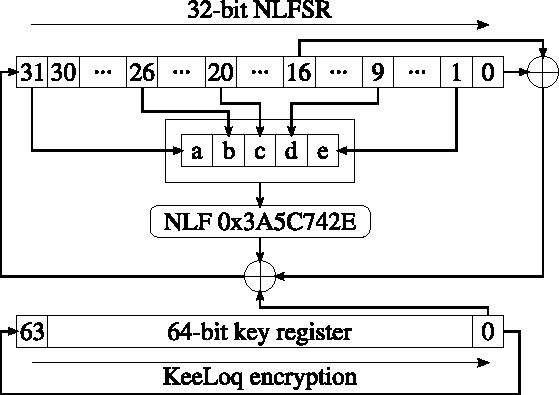
\includegraphics[width=\textwidth]{figures/KeeLoq-Encryption.pdf}
    \caption{Encryption.}
  \end{subfigure}
  \hfill
  \begin{subfigure}[b]{0.48\textwidth}
    \centering
    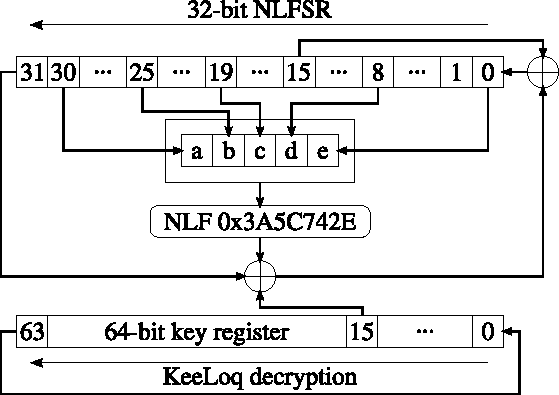
\includegraphics[width=\textwidth]{figures/KeeLoq-Decryption.pdf}
    \caption{Decryption.}
  \end{subfigure}
  \caption{KeeLoq round structure.
  The very small round function and the period 64 key schedule are the structural properties used by both attacks in this paper.}
  \label{fig:keeloq-round}
\end{figure}

\subsection{A Basic Key Extraction Fact}

The FP and S/MITM attacks rely on the following key extraction fact:
if two internal states of KeeLoq are known and separated by at most 32 rounds, the intervening key bits can be recovered directly.

\begin{lemma}\label{lem:linear-step}
Let $A$ and $B$ be two known internal states of KeeLoq such that $B$ is obtained from $A$ after $t$ forward rounds, where $t \leq 32$.
Then the $t$ key bits used in these rounds are uniquely determined by $(A,B)$ and can be recovered in time linear in $t$.
\end{lemma}

\begin{proof}
In one forward round the new feedback bit is
\[
\varphi = \NLF(s_{31}, s_{26}, s_{20}, s_9, s_1) \oplus s_{16} \oplus s_0 \oplus k.
\]
If the distance is at most 32 rounds, then at each step the new feedback bit appears at a known position of the later state.
Hence the round equation can be rearranged to solve for the corresponding key bit.
Repeating this for all $t$ rounds recovers the whole key fragment.
Uniqueness follows because each round equation fixes exactly one key bit once the two endpoint states are known.
\end{proof}

A round-indexed derivation is given in \autoref{app:proof-linear-step}.
This fact explains why both attacks peel 16 rounds first, and
why the meet-in-the-middle attack can recover key fragments from pairs of intermediate states rather than by brute force.

\subsection{The NLFSR Passthrough Property}\label{subsec:passthrough}

KeeLoq's round operation shifts the 32 bit state right by one position and injects a key dependent feedback bit at position~31.
After $t \leq 32$ forward rounds from state $A$ to state $B$, the result decomposes as
\[
B[31:32{-}t] = \text{new feedback bits (key dependent)},
\qquad
B[31{-}t:0] = A[31:t].
\]
The low $32-t$ bits of $B$ are \emph{passthrough copies} of the high $32-t$ bits of $A$ and require no key knowledge to compute.
Decryption reverses the shift (left by one, new bit at position~0), so after $t \leq 32$ backward rounds the high $32-t$ bits of $B$ are passthrough copies of the low $32-t$ bits of $A$.

For $t=16$:
\begin{itemize}
  \item \textbf{Forward.} $B[15:0] = A[31:16]$: the low 16~output bits are a free copy of the high 16~input bits.
  \item \textbf{Backward.} $B[31:16] = A[15:0]$: the high 16~output bits are a free copy of the low 16~input bits.
\end{itemize}
This passthrough structure is used by the 16 bit filter in the FP attack (\autoref{sec:fixedpoint}) and by the state construction in the S/MITM attack (\autoref{sec:mitm}).

\subsection{Cycle Terminology}\label{subsec:cycle-terminology}

We classify fixed points of $F^8$ by their cycle structure under $F$:
\begin{itemize}
  \item A \textbf{1-cycle} (or fixed point of $F$) is a state $S$ with $F(S) = S$.
  \item A \textbf{2-cycle} is a pair $(S_1,S_2)$ with $F(S_1)=S_2$ and $F(S_2)=S_1$.
  Both elements are fixed points of $F^2$ and hence of $F^8$.
  \item A \textbf{4-cycle} consists of four states $S_0 \to S_1 \to S_2 \to S_3 \to S_0$ under $F$.
  All four are fixed points of $F^4$ and hence of $F^8$.
  \item An \textbf{8-cycle} is an orbit of length~8 under $F$; all eight elements are fixed points of $F^8$.
\end{itemize}
Every fixed point of $F^8$ belongs to exactly one of these cycle types.
The cycle type determines how many true fixed points vote together in phase~1 and what kind of SAT constraints are available in phase~2.
This terminology explains which groups appear after phase~1 and why the exact recovery step depends on the underlying cycle type in \autoref{sec:fixedpoint}.

\subsection{A Heuristic Model for Cycle Structure}\label{subsec:heuristic-model}

The FP attack uses a standard heuristic assumption.

\begin{quote}
\textbf{Heuristic assumption.}
We model the 64 round permutation $F = E_{64}$ as a uniformly random permutation on $2^{32}$ points.
\end{quote}

This assumption is not a theorem about KeeLoq but a modeling choice;
the role of the experiments is to check whether the resulting predictions fit the observed data.

Under this model, the fixed points of $F^8$ are exactly the points that lie in cycles of length $1$, $2$, $4$, or $8$ of $F$.
Standard random permutation theory says that the number of $d$ cycles is approximately Poisson with mean $1/d$, and these random variables are asymptotically independent for fixed small $d$.
We write $\mathrm{Poi}(\lambda)$ for a Poisson random variable with mean parameter $\lambda$.
For convenience, basic Poisson facts used throughout the paper are summarized in
\autoref{app:poisson-basics}.

\begin{lemma}\label{lem:fp8-distribution}
Under the random permutation model for $F$, the number of fixed points of $F^8$ has distribution
\[
\mathrm{FP}_{F^8} = 1\cdot \mathrm{Poi}(1)
+ 2\cdot \mathrm{Poi}(1/2)
+ 4\cdot \mathrm{Poi}(1/4)
+ 8\cdot \mathrm{Poi}(1/8),
\]
where the four Poisson variables are asymptotically independent.
\end{lemma}

\begin{proof}
A point is fixed by $F^8$ if and only if it lies in a cycle of $F$ whose length divides $8$.
Thus only cycle lengths $1$, $2$, $4$, and $8$ matter.
A $d$ cycle contributes exactly $d$ fixed points to $F^8$.
The standard random permutation model gives the number of $d$ cycles as approximately $\mathrm{Poi}(1/d)$.
Summing the contributions of the relevant cycle lengths gives the claim.
\end{proof}

As a consequence, $\mathbb{E}[\mathrm{FP}_{F^8}] = 4$, $\mathrm{Var}[\mathrm{FP}_{F^8}] = 15$, and $\Pr[\mathrm{FP}_{F^8} = 0] = e^{-15/8} \approx 0.153$.
Hence the probability that at least one true fixed point exists is about $84.7\%$.
Conditional on such a point, phase~2 enumerates every directed mapping or singleton completion needed for recovery.
The implementation therefore has the same end-to-end success probability under the model.
The expectation and variance computation is expanded in \autoref{app:proof-fp8-moments}.
This heuristic model predicts the success probability and the spread in the number of useful fixed points across keys in \autoref{sec:fixedpoint}, and later supports comparison with the benchmark data.

\paragraph{Large Variation.}
The variance $15$ corresponds to a standard deviation of $\sqrt{15}\approx3.87$, so the fixed-point count is substantially more dispersed than a $\mathrm{Poi}(4)$ variable, whose variance is $4$.
The extra dispersion comes from longer cycles: one 8-cycle of $F$ contributes 8~fixed points of $F^8$ at once, so some keys have many more fixed points than others.
This matters in practice because the number of true fixed points can vary a lot across keys, from zero to 18 or more in our experiments.

\subsection{GPU Measurement Platform}\label{subsec:gpu-platform}

Unless stated otherwise, the revised GPU measurements use one NVIDIA RTX PRO~6000 Blackwell Workstation Edition with compute capability 12.0, 188 streaming multiprocessors, 97,887~MiB of device memory, and a 500~W board limit.
The system ran Linux 6.8.0-49-generic with NVIDIA driver 590.48.01 and CUDA~12.8, and the CUDA targets were compiled for \texttt{sm\_120}.
We report direct measurements for brute force and the fixed-point experiment.
For S/MITM, we measure a complete bounded scan of 64 low-key prefixes and explicitly label the corresponding full-$2^{16}$ scan times as extrapolations.
The Apple M4 CPU measurement reported later is unchanged from the original submission.

\section{A GPU Brute-Force Baseline (BF)}\label{sec:bruteforce}

Brute force is the baseline for KeeLoq.
It uses no structural assumption and covers the whole key space.
With two known plaintext ciphertext pairs, a wrong key survives both tests with probability about $2^{-64}$ under the standard random permutation heuristic.
So two pairs identify the correct 64-bit key with overwhelming probability, and the main question is search rate.

\subsection{GPU Basics and Terms}

A CUDA kernel is launched as a \emph{grid} of \emph{thread blocks}.
Each block contains many \emph{threads}, and the hardware assigns blocks to streaming multiprocessors, or SMs.
Threads inside one block can synchronize and share on-chip resources, while different blocks are independent and may run in any order.
For brute force, this matches the problem well because one candidate key can be tested independently of every other candidate key.

In our implementation, the launch is one-dimensional.
If a kernel uses $B$ threads per block and $G$ blocks, then the launch creates $G \cdot B$ logical threads.
In CUDA notation, these are $\mathtt{blockDim.x}=B$ and $\mathtt{gridDim.x}=G$.
Thread $t$ gets the global index
\[
t = \mathtt{blockIdx.x} \cdot \mathtt{blockDim.x} + \mathtt{threadIdx.x},
\]
and this index determines which candidate key range it scans.
So the hierarchy is simple: the grid is the full launch, each block is one independent group inside that launch, and each thread is one worker inside a block.
\autoref{fig:gpu-execution-model} illustrates this mapping.

A warp is a group of 32 threads that the hardware issues together.
The 192-thread blocks in our main benchmark therefore contain 6 warps each.
The SM keeps several warps ready and switches among them to hide latency.
Occupancy measures how many warps are available to run relative to the hardware limit, but high occupancy alone is not enough: the kernel must also keep its hot path short and avoid unnecessary memory traffic.

KeeLoq brute-force search is a good GPU workload because each thread does almost the same work and needs very little memory.
Registers are the fastest storage on the device, so we keep the state, the candidate key, and the two plaintext-ciphertext pairs in registers.
\autoref{fig:gpu-memory-hierarchy} summarizes the memory scopes relevant here: registers are thread-private, shared memory is block-local, and global memory is device-wide.
Each thread then checks its assigned keys locally, and only the rare survivors need to be reported back to the host.
Performance therefore depends mainly on how efficiently the kernel turns candidate keys into integer instructions while keeping enough warps ready on each SM.

\begin{figure}[htbp]
\centering
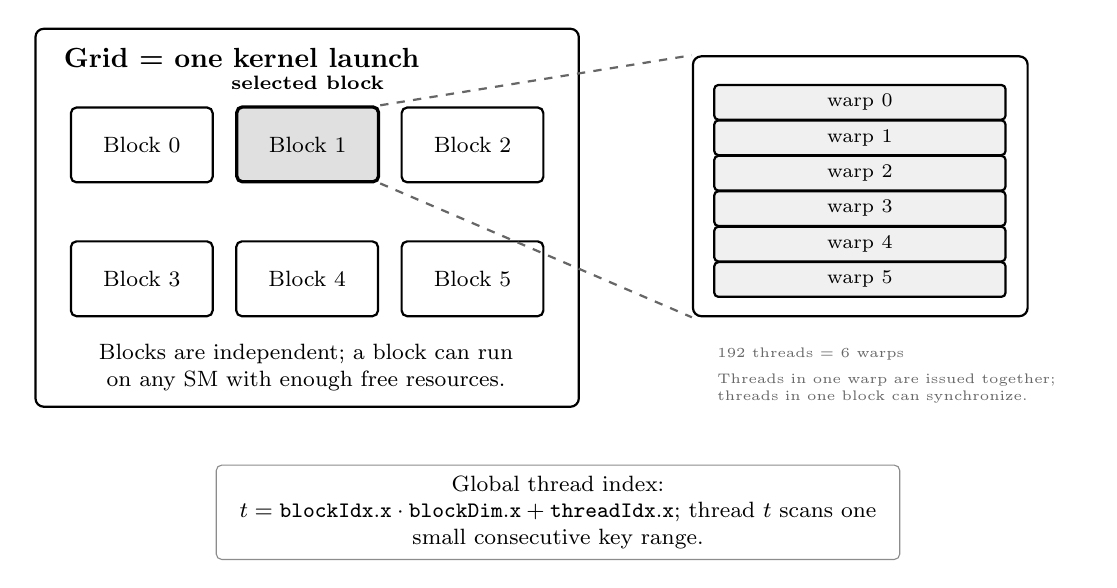
\begin{tikzpicture}[
  x=1cm,y=1cm,
  font=\footnotesize,
  >=Stealth,
  panel/.style={rounded corners=3pt, draw=black, fill=white, thick},
  block/.style={rounded corners=2pt, draw=black, fill=white, thick,
                minimum width=1.8cm, minimum height=0.95cm, align=center, inner sep=3pt},
  selected/.style={rounded corners=2pt, draw=black, fill=black!12, very thick,
                   minimum width=1.8cm, minimum height=0.95cm, align=center, inner sep=3pt},
  warpbar/.style={rounded corners=1.5pt, draw=black, fill=black!6, thick,
                  minimum width=3.7cm, minimum height=0.34cm, anchor=west, align=center},
  note/.style={align=left, text=black, inner sep=1pt},
  footerbox/.style={rounded corners=2pt, draw=black!45, fill=white, inner sep=4pt}
]
  \node[panel, minimum width=6.9cm, minimum height=4.8cm, anchor=south west] (grid) at (0,0) {};
  \node[anchor=west, text=black, font=\bfseries] at (0.25,4.45) {Grid = one kernel launch};

  \node[block, anchor=south west] (b0) at (0.45,2.85) {Block 0};
  \node[selected, anchor=south west] (b1) at (2.55,2.85) {Block 1};
  \node[block, anchor=south west] (b2) at (4.65,2.85) {Block 2};
  \node[block, anchor=south west] (b3) at (0.45,1.15) {Block 3};
  \node[block, anchor=south west] (b4) at (2.55,1.15) {Block 4};
  \node[block, anchor=south west] (b5) at (4.65,1.15) {Block 5};
  \node[anchor=south, text=black, font=\scriptsize\bfseries] at ($(b1.north)+(0,0.08)$) {selected block};

  \node[note, anchor=south, text width=7cm, align=center] at (3.45,0.18)
    {Blocks are independent; a block can run on any SM with enough free resources.};

  \node[panel, minimum width=4.25cm, minimum height=3.30cm, anchor=south west] (zoom) at (8.35,1.15) {};
  \node[anchor=north west, text=black!60, font=\tiny] at (8.55,0.88)
    {192 threads = 6 warps};

  \draw[dashed, draw=black!60, thick] (b1.north east) -- (zoom.north west);
  \draw[dashed, draw=black!60, thick] (b1.south east) -- (zoom.south west);

  \foreach \i in {0,...,5} {
    \pgfmathsetmacro{\y}{3.88 - 0.45*\i}
    \node[warpbar, text=black, font=\scriptsize] (w\i) at (8.62,\y) {warp \i};
  }

  \node[anchor=north west, text=black!60, font=\tiny, text width=4.6cm] at (8.55,0.55)
    {Threads in one warp are issued together; threads in one block can synchronize.};

  \node[footerbox, anchor=north] at (6.65,-0.72) {
    \begin{minipage}{8.4cm}
    \centering
    Global thread index:\\
    $t = \mathtt{blockIdx.x}\cdot\mathtt{blockDim.x}+\mathtt{threadIdx.x}$; thread $t$ scans one small consecutive key range.
    \end{minipage}
  };
\end{tikzpicture}
\caption{CUDA execution model for the brute-force kernel.
The left panel shows the grid and its thread blocks; the right panel zooms into one 192-thread block and its 6 warps.
Each thread uses its global index to scan a small consecutive key range.}
\label{fig:gpu-execution-model}
\end{figure}

\begin{figure}[htbp]
\centering
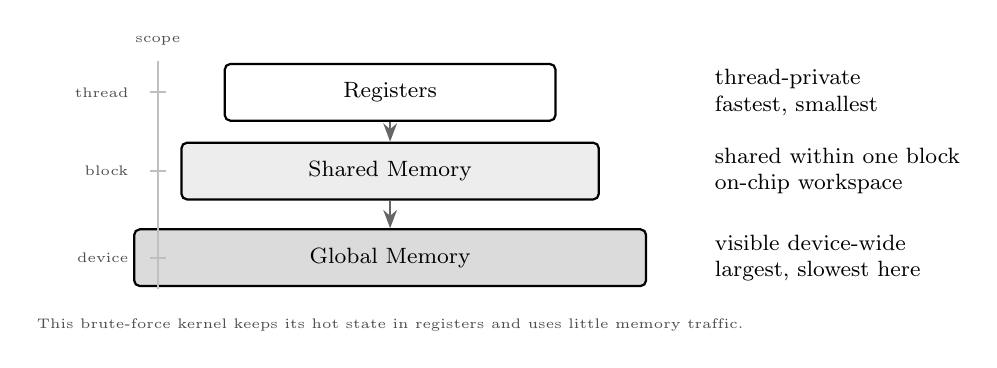
\begin{tikzpicture}[
  x=1cm,y=1cm,
  font=\footnotesize,
  >=Stealth,
  mem/.style={rounded corners=2pt, thick, minimum height=0.72cm, align=center},
  reg/.style={mem, draw=black, fill=white, minimum width=4.2cm},
  shr/.style={mem, draw=black, fill=black!7, minimum width=5.3cm},
  glob/.style={mem, draw=black, fill=black!14, minimum width=6.5cm},
  side/.style={text=black, align=left},
  cue/.style={text=black!70, align=center}
]
  \node[reg] (reg) at (0,1.95) {Registers};
  \node[shr] (shr) at (0,0.95) {Shared Memory};
  \node[glob] (glob) at (0,-0.15) {Global Memory};

  \draw[->, thick, draw=black!60] (reg.south) -- (shr.north);
  \draw[->, thick, draw=black!60] (shr.south) -- (glob.north);

  \node[side, anchor=west] at (4.0,1.95) {thread-private\\fastest, smallest};
  \node[side, anchor=west] at (4.0,0.95) {shared within one block\\on-chip workspace};
  \node[side, anchor=west] at (4.0,-0.15) {visible device-wide\\largest, slowest here};

  \node[cue, font=\tiny, anchor=south] at (-2.95,2.42) {scope};
  \node[cue, font=\tiny, anchor=east] at (-3.2,1.95) {thread};
  \node[cue, font=\tiny, anchor=east] at (-3.2,0.95) {block};
  \node[cue, font=\tiny, anchor=east] at (-3.2,-0.15) {device};

  \draw[thick, draw=black!25] (-2.95,2.35) -- (-2.95,-0.55);
  \draw[thick, draw=black!25] (-3.05,1.95) -- (-2.85,1.95);
  \draw[thick, draw=black!25] (-3.05,0.95) -- (-2.85,0.95);
  \draw[thick, draw=black!25] (-3.05,-0.15) -- (-2.85,-0.15);

  \node[cue, font=\tiny, anchor=north] at (0,-0.8) {This brute-force kernel keeps its hot state in registers and uses little memory traffic.};
\end{tikzpicture}
\caption{Simplified CUDA memory scope for the brute-force kernel.
Registers are thread-private, shared memory is block-local, and global memory is device-wide.
The hot state stays in registers.}
\label{fig:gpu-memory-hierarchy}
\end{figure}

\subsection{Attack Structure}

The BF attack is straightforward.
For each candidate key $K$, we check whether
\[
E_{528}(K,P_0)=C_0
\quad\text{and}\quad
E_{528}(K,P_1)=C_1.
\]
The first pair rejects almost every wrong key.
The second pair is used only for the tiny number of survivors.
Hence the expected work per tested key is $1 + 2^{-32}$
full encryptions, which is essentially one encryption per key.

\begin{algorithm}[htbp]
\caption{GPU brute-force search for KeeLoq}\label{alg:bruteforce}
\SetAlgoLined
\KwIn{Two plaintext-ciphertext pairs $(P_0,C_0)$ and $(P_1,C_1)$}
\KwOut{The 64-bit key or failure}
partition the key space into GPU-sized chunks\;
\For{each chunk}{
  launch a GPU kernel over all candidate keys in the chunk\;
  \ForPar{each candidate key $K$ assigned to one thread}{
    \If{$E_{528}(K,P_0) \neq C_0$}{
      continue\;
    }
    \If{$E_{528}(K,P_1) = C_1$}{
      emit $K$ as a candidate key\;
    }
  }
  stop when the host verifies a returned key\;
}
\Return failure if no chunk returns a valid key\;
\end{algorithm}

Our implementation also supports fixed masks such as \texttt{--fix-low}.
We use that mode for benchmarking because it lets us run a controlled subspace such as $2^{40}$ keys while still exercising the same hot path as a full search.

\subsection{Implementation Features}

The implementation combines data-level parallelism with reductions in the per-round instruction count.

\begin{itemize}
  \item We use a contiguous key path for the common case where the free key bits form one interval.
  In that path, each thread constructs candidate keys with one shift and one OR, which keeps the hot path short.
  \item We use a 32-lane bit-sliced layout inside each thread.
  A 32-bit machine word then carries one bit from 32 candidate keys at once, so one sequence of Boolean operations advances 32 keys in parallel.
  \item We exploit the exhaustively verified identity
  $\NLF(e,d,c,b,a)=\NLF(e,0,c\oplus d,b\oplus d,a\oplus d)$.
  It replaces the generic nonlinear-function multiplexer with three XOR and three ternary-logic operations.
  \item We rotate state indices rather than moving all 32 state words after each round.
  Loop unrolling makes every rotated index a compile-time constant.
  \item We keep the waterfall test inside one kernel.
  Each candidate key is tested on the first pair first, and the second pair is evaluated only for the rare survivors.
  This avoids a second kernel launch and makes the effective cost almost one encryption per key.
  \item At round~512, we compare the 16 ciphertext bits already fixed by the passthrough property.
  This rejects all 32 lanes with probability $(1-2^{-16})^{32}\approx0.9995$, allowing almost every candidate batch to skip the final 16 rounds.
  \item We use \texttt{\_\_launch\_bounds\_\_(192,2)} so the compiler's register allocation supports two resident blocks per streaming multiprocessor.
\end{itemize}

The main speedup came from the bit slice restructuring.
In the KeeLoq kernel, one thread handles 32 candidates at once.
For round $r$ and state bit $b$, let $y^{(r,\ell)}_b$ be bit $b$ of lane $\ell$, where $0 \leq \ell < 32$, and pack that bit-plane as $X_b^{(r)} = \sum_{\ell=0}^{31} y_b^{(r,\ell)} 2^\ell$.
The round-key bit is packed as $K_r = \sum_{\ell=0}^{31} k_{r \bmod 64}^{(\ell)} 2^\ell$.
The kernel therefore computes the KeeLoq feedback bit itself in bit-sliced form,
\[
F^{(r)} = \NLF_{\mathrm{bs}}\!\bigl(X_{31}^{(r)}, X_{26}^{(r)}, X_{20}^{(r)}, X_9^{(r)}, X_1^{(r)}\bigr)
\oplus X_{16}^{(r)} \oplus X_0^{(r)} \oplus K_r,
\]
where $\NLF_{\mathrm{bs}}$ is the same KeeLoq nonlinear function as in the scalar cipher, evaluated lane-wise on 32 lanes at once.
The implementation realizes it directly from the KeeLoq lookup constant $\mathtt{0x3A5C742E}$ rather than from a memory table.
The state update is the KeeLoq shift:
\[
X_{31}^{(r+1)} = F^{(r)},
\qquad
X_b^{(r+1)} = X_{b+1}^{(r)} \quad (0 \leq b < 31).
\]
One sequence of word-level Boolean instructions therefore executes one full KeeLoq round for 32 candidate keys in parallel.
In the contiguous-key kernel, the 32 lanes correspond to consecutive candidates, so only the lowest five free key bits differ across lanes and the higher key planes are shared.

\subsection{Benchmark Results}\label{sec:bruteforce-experimental}

We measured three consecutive runs on the platform described in \autoref{subsec:gpu-platform}.
The optimized full-round contiguous kernel used 192-thread blocks, eight inner-loop bits, and a launch bound of two resident blocks per SM.
To keep the run short but still meaningful, we fixed 24 low key bits and searched the remaining $2^{40}$ candidates.
The target key was found after $37.5\%$ of that search space.
The three throughputs were 177.527, 176.909, and 176.284~Gkeys/s, a spread of $0.7\%$.
The median is 176.909~Gkeys/s, or about $2^{37.36}$ keys/s.
The derived search times in \autoref{tab:bruteforce-benchmark} use this median run.

\begin{table}[htbp]
  \centering
  \caption{RTX PRO~6000 brute-force benchmark.}
  \label{tab:bruteforce-benchmark}
  \footnotesize
  \setlength{\tabcolsep}{3pt}
  \renewcommand{\arraystretch}{1.05}
  \begin{tabular}{@{}lrrrrr@{}}
    \toprule
    GPU & \shortstack{Throughput\\(Gkeys/s)} & \shortstack{Keys\\tested} & \shortstack{Kernel\\time (s)} & \shortstack{Expected search\\(years)} & \shortstack{Worst-case search\\(years)} \\
    \midrule
    RTX PRO~6000 & 176.909 & 412,316,860,416 & 2.331 & 1.65 & 3.30 \\
    \bottomrule
  \end{tabular}
\end{table}

To isolate the effect of the implementation changes from the change of hardware, we also ran the submitted and revised kernels on the same RTX PRO~6000 with identical commands and build flags.
Throughput increased from 131.011 to 174.516~Gkeys/s, a factor of $1.33$.
The final 176.909~Gkeys/s median above comes from a separate three-run measurement of the revised code.

From the measured single-GPU rate, we extrapolate the idealized cluster-scale times in \autoref{tab:bruteforce-scaling}.
The calculation assumes linear scaling because candidate keys are independent, but it excludes all system and communication overhead.
At this rate, a one-week worst-case search requires 173 GPUs and a one-day search requires 1,207 GPUs.

\begin{table}[htbp]
  \centering
  \caption{Idealized multi-GPU brute-force scaling.}
  \label{tab:bruteforce-scaling}
  \setlength{\tabcolsep}{4pt}
  \renewcommand{\arraystretch}{1.05}
  \begin{tabular}{@{}lrr@{}}
    \toprule
    GPU count & Worst-case time (h) & Expected time (h) \\
    \midrule
    1 & 28,965 & 14,482 \\
    8 & 3,621 & 1,810 \\
    41 & 707 & 353 \\
    173 & 167.4 & 83.7 \\
    1,207 & 24.0 & 12.0 \\
    \bottomrule
  \end{tabular}
\end{table}

These figures are GPU-only lower bounds.
They do not include host servers, memory, storage, networking, racks, cooling, power delivery, electricity, or acquisition cost.

This baseline matters for the rest of the paper.
A structural attack should be judged not only by its asymptotic complexity, but also by whether it beats this measured brute-force rate under its own data assumptions.
We next turn to structural attacks that do beat brute force once their data conditions hold.

\section{A Full-Codebook Fixed-Point Attack}\label{sec:fixedpoint}

\subsection{Main Idea}

The FP attack starts from the identity $E_{528} = E_{16} \circ F^8$.
If a plaintext $P$ is a fixed point of $F^8$, then the full encryption reduces to 16 rounds.

\begin{lemma}[Fixed point reduction]\label{lem:fixedpoint-reduction}
If $P$ is a fixed point of $F^8$, then
\[
E_{528}(K,P) = E_{16}(K,P).
\]
\end{lemma}

\begin{proof}
By definition, $F^8(P)=P$.
Since $E_{528}=E_{16}\circ F^8$, we get
\[
E_{528}(K,P) = E_{16}(K,F^8(P)) = E_{16}(K,P).
\]
\end{proof}

This lemma turns a 528 round relation into a 16 round relation on the same plaintext.
The attack uses this fact in two phases.
In phase~1, we scan the full plaintext space and retain pairs $(P,C)$ that are consistent with a 16-round encryption.
In phase 2 we use the surviving candidates to recover the remaining 48 key bits.

\begin{figure}[htbp]
\centering
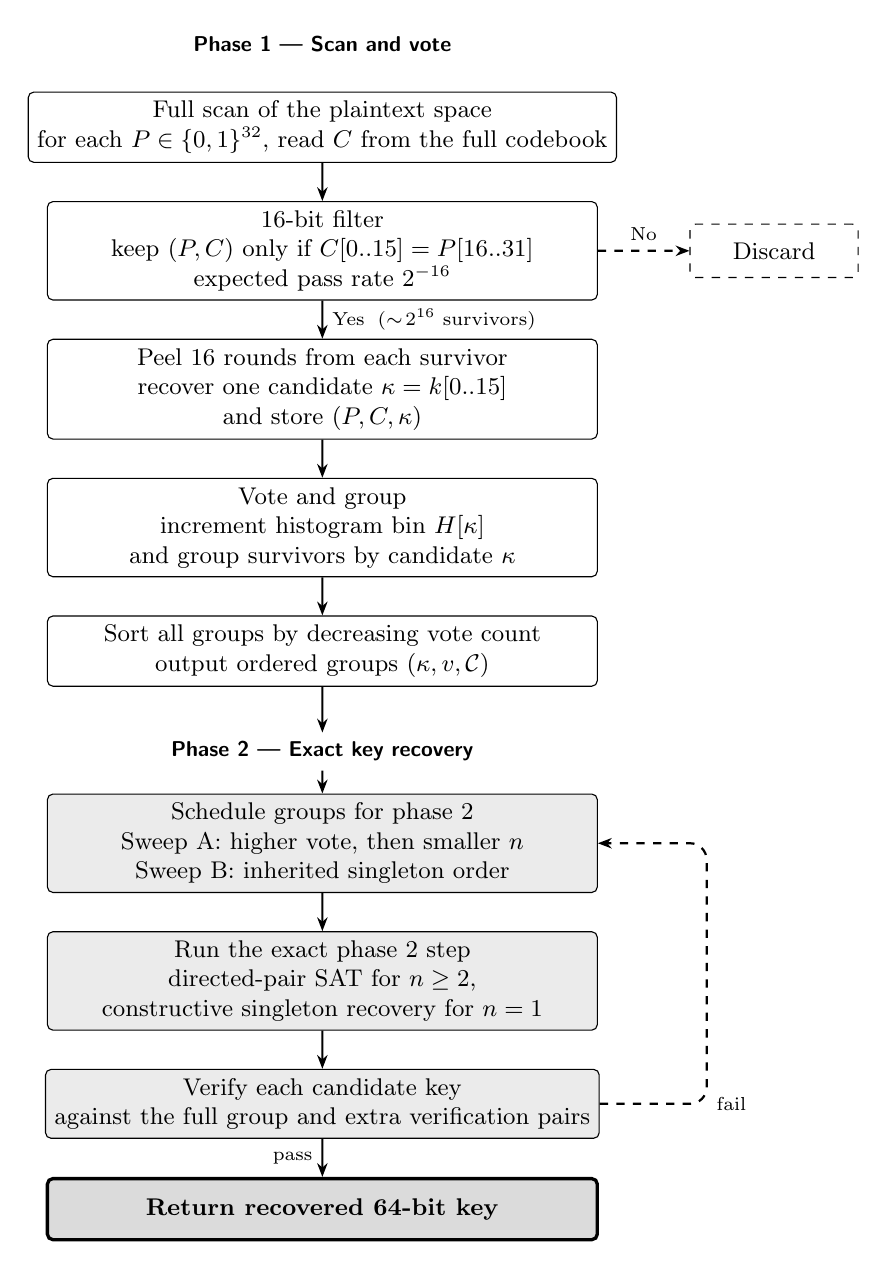
\begin{tikzpicture}[scale=0.97, transform shape,
  node distance=5mm and 6mm,
  box/.style={rectangle, rounded corners=2pt, draw=black, fill=white,
              minimum width=7.2cm, minimum height=8mm,
              align=center, font=\small},
  phasebox/.style={box, fill=black!8},
  resultbox/.style={box, fill=black!14, very thick},
  discard/.style={rectangle, rounded corners=2pt, draw=black, fill=white, dashed,
                  minimum height=7mm, align=center, font=\small},
  lbl/.style={font=\footnotesize\bfseries, text=black},
  arr/.style={-{Stealth[length=5pt]}, thick},
  darr/.style={-{Stealth[length=5pt]}, thick, dashed, draw=black},
  note/.style={font=\scriptsize, text=black},
]
  % ---- Phase 1 ----
  \node[lbl] (p1) {\textsf{Phase~1 --- Scan and vote}};
  \node[box, below=4mm of p1] (scan)
      {Full scan of the plaintext space\\
      for each $P \in \{0,1\}^{32}$, read $C$ from the full codebook};
  \node[box, below=of scan] (filt)
      {16-bit filter\\
       keep $(P,C)$ only if $C[0..15] = P[16..31]$\\
      expected pass rate $2^{-16}$};
  \node[discard, right=12mm of filt, minimum width=2.2cm] (disc) {Discard};
  \node[box, below=of filt] (peel)
      {Peel 16 rounds from each survivor\\
       recover one candidate $\kappa = k[0..15]$\\
      and store $(P,C,\kappa)$};
  \node[box, below=of peel] (vote)
      {Vote and group\\
       increment histogram bin $H[\kappa]$\\
      and group survivors by candidate $\kappa$};
  \node[box, below=of vote] (rank)
      {Sort all groups by decreasing vote count\\
       output ordered groups $(\kappa, v, \mathcal{C})$};

  % ---- Phase 2 ----
    \node[lbl, below=6mm of rank] (p2) {\textsf{Phase~2 --- Exact key recovery}};
    \node[phasebox, below=3mm of p2] (pick)
      {Schedule groups for phase~2\\
       Sweep~A: higher vote, then smaller $n$\\
       Sweep~B: inherited singleton order};
  \node[phasebox, below=of pick] (sat)
      {Run the exact phase~2 step\\
       directed-pair SAT for $n\geq 2$,\\
      constructive singleton recovery for $n=1$};
  \node[phasebox, below=of sat] (verify)
      {Verify each candidate key\\
       against the full group and extra verification pairs};
  \node[resultbox, below=of verify]
       (done) {\textbf{Return recovered 64-bit key}};

  % ---- Phase 1 arrows ----
  \draw[arr] (scan) -- (filt);
  \draw[darr] (filt) -- node[above, font=\scriptsize]{No} (disc);
  \draw[arr] (filt) -- node[right, note]{Yes\; ($\sim\!2^{16}$ survivors)} (peel);
  \draw[arr] (peel) -- (vote);
  \draw[arr] (vote) -- (rank);

  % ---- Phase transition ----
  \draw[arr] (rank) -- (p2);
  \draw[arr] (p2) -- (pick);

  % ---- Phase 2 arrows ----
  \draw[arr] (pick) -- (sat);
  \draw[arr] (sat) -- (verify);
  \draw[arr] (verify) -- node[left, font=\scriptsize]{pass} (done);

  % ---- Fail loop: clean right-side arc from verify back to pick ----
  \draw[darr, rounded corners=6pt]
    (verify.east) -- ++(14mm,0)
    node[right, note]{fail}
    |- (pick.east);
\end{tikzpicture}
\caption{Workflow of the fixed-point attack.
Light gray distinguishes the exact-recovery phase; dashed arrows denote rejection or retry paths.}
\label{fig:fixedpoint-workflow}
\end{figure}

\subsection{Phase 1}

Let $P$ be a plaintext and let $C = E_{528}(K,P)$.
If $P$ is a true fixed point of $F^8$, then by \autoref{lem:fixedpoint-reduction} we have $C = E_{16}(K,P)$.
By the passthrough property (\autoref{subsec:passthrough}), every true fixed point must satisfy
$C[0..15] = P[16..31].$
A random pair passes this filter with probability $2^{-16}$.
Thus, when we scan all $2^{32}$ plaintexts, we expect about $2^{16}$ false positives and at most a small number of true fixed points (typically 2 to 8 when they exist).

For every survivor of the filter, phase~1 uses \autoref{lem:linear-step} to peel 16 rounds and recover a candidate for the low 16 key bits $k[0..15]$.

\paragraph{How peeling works.}
The filter already confirms $C[0..15] = P[16..31]$, so the low 16 output bits carry no new information.
The high 16 bits of $C$ are the 16 feedback bits from rounds~0 to~15:
$C[16+i]$ is the feedback bit $\varphi_i$ from round~$i$.
Since we know both $P$ and $C$, we can recover each key bit by rearranging the round equation:
\[
k_i = C[16+i] \oplus \NLF(s_{31},s_{26},s_{20},s_9,s_1) \oplus s_{16} \oplus s_0,
\]
where $s$ is the running state after $i$ rounds from $P$.
The algorithm is:
\begin{enumerate}
  \item Set $s^{(0)} \leftarrow P$.
  \item For $i = 0, 1, \ldots, 15$:
  \begin{enumerate}
    \item compute $\mathit{nlf} = \NLF(s^{(i)}_{31}, s^{(i)}_{26}, s^{(i)}_{20}, s^{(i)}_9, s^{(i)}_1)$;
    \item read the known feedback bit $\mathit{fb} = C[16+i]$;
    \item solve for the key bit: $k[i] = \mathit{fb} \oplus \mathit{nlf} \oplus s^{(i)}_{16} \oplus s^{(i)}_0$;
    \item advance the state: $s^{(i+1)} \leftarrow (s^{(i)} \gg 1) \mid (\mathit{fb} \ll 31)$.
  \end{enumerate}
\end{enumerate}
This recovers the full 16~bit candidate $k[0..15]$ using only XOR operations, without brute force.

\paragraph{How voting works.}
We use the following terminology throughout both phases.
A \emph{survivor} is a pair $(P,C)$ that passes the 16-bit filter, and peeling assigns it one candidate value $\kappa$ for $k[0..15]$.
The \emph{bin} indexed by $\kappa$ has count $H[\kappa]$.
The corresponding \emph{group} $G[\kappa]$ is the actual list of survivors assigned to that bin, so $|G[\kappa]|=H[\kappa]$.
The \emph{true bin} is indexed by the correct fragment $\kappa^{\star}=k[0..15]$; every true fixed point of $F^8$ belongs to its group.
Every other bin is a \emph{false bin}, and survivors produced only by the random filter are \emph{false survivors}.
A false survivor can also land in the true bin by chance.
For example, three true fixed points and two accidental survivors with peeled value $\kappa^{\star}$ give a true-group count of five.

Phase~1 produces approximately $2^{16}$ false survivors whose peeled values are modeled as uniform over $2^{16}$ bins.
The expected false load per bin is therefore approximately one, modeled by $\mathrm{Poi}(1)$.
The largest false-bin count is typically between 7 and 9.
A true bin with at least 8 votes is therefore usually ranked first, whereas a smaller count can place it behind many false bins.

\begin{algorithm}[htbp]
\caption{Phase 1 of the FP attack}\label{alg:fixedpoint-phase1}
\SetAlgoLined
\KwIn{The full plaintext space $\{0,1\}^{32}$}
\KwOut{A survivor list $L$ and candidate groups $(G[\kappa])_{\kappa \in \{0,1\}^{16}}$ ordered by decreasing $H[\kappa]$}
Initialize $L \gets [\,]$\;
\For{each plaintext $P \in \{0,1\}^{32}$}{
  compute $C = E_{528}(K,P)$\;
  \If{$C[0..15] = P[16..31]$}{
    peel 16 rounds from $(P,C)$ to recover a candidate $\kappa \in \{0,1\}^{16}$\;
    append $(P,C,\kappa)$ to $L$\;
  }
}
Initialize $H[\kappa] \gets 0$ for all $\kappa \in \{0,1\}^{16}$\;
\For{each $(P,C,\kappa) \in L$}{
  set $H[\kappa] \gets H[\kappa] + 1$\;
}
Sort the indices $\kappa \in \{0,1\}^{16}$ by decreasing vote count $H[\kappa]$\;
\For{each $\kappa \in \{0,1\}^{16}$}{
  set $G[\kappa] \gets [(P,C) : (P,C,\kappa) \in L]$\;
}
\Return{$L$, the ordered family $(G[\kappa])_{\kappa \in \{0,1\}^{16}}$, and the counts $H[\kappa]$}\;
\end{algorithm}

The crucial point is that phase~1 keeps all groups, sorted by vote count, not just the top ranked one.
As noted above, the correct group may rank anywhere from first to tens of thousands depending on the number of true fixed points.
Phase~2 visits groups in decreasing vote order until a valid key is found.

Under the Poisson occupancy approximation, \autoref{tab:rank-distribution} quantifies this tradeoff.
Let $B = 2^{16}$ be the number of candidate bins for $k[0..15]$, one bin for each possible 16-bit value of the peeled key fragment.
Let $F$ be the total number of false survivors produced by phase~1.
For each false bin $b \neq b^{\star}$, let $X_b$ be the number of false survivors assigned to $b$, where $b^{\star}$ denotes the true bin.
Under the standard Poisson occupancy model, we approximate the false-bin loads $X_b$ as independent $\mathrm{Poi}(\lambda)$ random variables with mean $\lambda = F/(B-1)$.
In our setting $F \approx 2^{16}$ and $B-1 = 2^{16}-1$, so $\lambda$ is extremely close to $1$.
Thus the number of false bins with $\geq k$ votes can be computed directly from the Poisson tail.
See \autoref{app:poisson-basics} for the basic formulas.
Approximating $\lambda$ by $1$, if $X \sim \mathrm{Poi}(1)$, then
\[
\Pr[X \geq k] = 1 - e^{-1}\sum_{j=0}^{k-1} \frac{1}{j!}
= e^{-1}\sum_{j=k}^{\infty} \frac{1}{j!}.
\]
Hence the expected number of false bins with at least $k$ votes is $(B-1) \cdot \Pr[X \geq k]$.
If the true bin has exactly $k$ votes, let $R(k)$ denote its expected rank in the vote-ordered list.
All false bins with more than $k$ votes are ahead of it, while half of the false bins tied at $k$ votes precede it on average.
Under the Poisson model, this gives
\[
R(k) \;\approx\; 1 + (B-1)\Pr[X \geq k+1] + \frac{1}{2}(B-1)\Pr[X = k].
\]
The table uses this tie-corrected estimate.
The approximation comes from replacing the finite occupancy distribution by independent Poisson loads; conditional on that model, the displayed rank is the tie-averaged expectation.
It shows that 8~votes already give expected rank about $1.4$, while 9~votes are essentially rank~1; by contrast, 5~votes still leave the true bin around rank~140 on average.

\begin{table}[htbp]
  \centering
  \caption{Expected true-bin rank by exact vote count.}
  \label{tab:rank-distribution}
  \setlength{\tabcolsep}{10pt}
  \begin{tabular}{ccc}
    \toprule
    True votes $k$ & Expected false bins & Expected rank \\
    \midrule
    5 & $\sim 240$ & $\sim 140$ \\
    6 & $\sim 39$ & $\sim 23$ \\
    7 & $\sim 5.5$ & $\sim 4.1$ \\
    8 & $\sim 0.67$ & $\sim 1.4$ \\
    9 & $\sim 0.07$ & $\sim 1.0$ \\
    \bottomrule
  \end{tabular}
\end{table}

The current 100-key benchmark is consistent with this heuristic.
Let $v^{\star}$ denote the vote count of the true bin.
For keys with $v^{\star}=5,6,7$, the observed mean ranks were $178$, $17.7$, and $3.1$, compared with the predicted values $140.4$, $23.2$, and $4.1$ from \autoref{tab:rank-distribution}; every benchmark key with $v^{\star} \geq 8$ ranked first.
For smaller vote counts, the same benchmark gave observed mean ranks about $3.2 \times 10^4$ for 1 vote, $1.13 \times 10^4$ for 2 votes, $3.28 \times 10^3$ for 3 votes, and $714$ for 4 votes, which matches the intended qualitative message that bins with only a few true votes are usually buried deep among false positives.

For the 15 absent keys ($v^{\star} = 0$) in our 100~key benchmark, the best false positive bin had 7~votes in 11 cases, 8~in 3 cases, and 9~in one case.
This confirms that the false positive noise floor is typically 7 and occasionally reaches 8 or 9, exactly as predicted by the $\mathrm{Poi}(1)$ model.

\subsection{Phase 2}

Once a candidate value for $k[0..15]$ is fixed, each survivor $(P,C)$ gives a known intermediate state
\[
M_{16} = E_{16}(k[0..15],P).
\]
The remaining unknown part is the upper 48 key bits
\[
k^{+} = k[16..63],
\]
which controls the remaining 48 rounds.

Phase~2 works one phase-1 group at a time.
Write one group as
\[
G = (\kappa, v, \mathcal{C}),
\qquad
\mathcal{C} = \{(P_i, C_i, M_i)\}_{i=1}^{n},
\]
where $\kappa$ is the candidate value of $k[0..15]$, $v$ is the vote count, and $n$ is the number of survivors in the group.
Here each
\[
M_i = E_{16}(\kappa,P_i)
\]
is known from phase~1.
We call a group with $n=1$ a \emph{singleton group}.
Each surviving phase-1 pair contributes exactly one vote to exactly one group, so $v=n$ for every group; in particular, every singleton group has $v=n=1$.

For one group, the goal is to decide whether some value of $k^{+}$ makes the group internally consistent.
We write one 48 round relation as
\[
\Phi_{i \to j}(k^{+}) : E_{48}(k^{+}, M_i) = P_j,
\]
meaning that $M_i$ maps to $P_j$ under the unknown 48-round suffix.

The implementation uses a small extra verification set
\[
\mathcal{V} = \{(P_t^{\mathrm{ext}}, C_t^{\mathrm{ext}})\}
\]
sampled from other groups.
A candidate key is accepted only if it satisfies the current group and also verifies on $\mathcal{V}$.

\paragraph{Sweep~A: exhaustive directed-pair SAT for groups with at least two candidates.}
If a group has $n \geq 2$ candidates, phase~2 fixes source indices $0$ and $1$ and tries all directed target pairs
\[
\Phi_{0 \to b}(k^{+}),\qquad \Phi_{1 \to d}(k^{+})
\qquad\text{for all } b,d \in \{0,\dots,n-1\}.
\]
The $n^2$ sweep covers 1-cycles, 2-cycles, 4-cycles, and 8-cycles uniformly.
For a false group, every pair of constraints is inconsistent and the solver rejects it.
For the true group with $n \geq 2$, the correct successor pair appears in the sweep, so recovery is certain.
The implementation schedules Sweep~A groups by decreasing vote count and, among equal-vote ties, prefers smaller groups first because their directed pair cost is about $n^2$.

\paragraph{Why two constraints suffice.}
One 48-round constraint gives 32~equations in 48 unknowns, so the random-function heuristic leaves about $2^{48-32}=2^{16}$ candidate keys.
Two independent constraints give 64 equations, reducing the expected number of spurious keys to $2^{48-64}=2^{-16}$.
So once the correct directed successor pair is tried, a group with $n \ge 2$ is usually solved uniquely.
This is a counting heuristic, not a theorem about KeeLoq.

\paragraph{Sweep~B: exact singleton recovery.}
If Sweep~A finds nothing, then the true group must be a singleton.
In that case, the group corresponds to a 1-cycle and satisfies
\[
\Phi_{0 \to 0}(k^{+}) : E_{48}(k^{+}, M_0) = P_0.
\]
This single constraint leaves exactly $2^{16}$ residual degrees of freedom.
Instead of enumerating SAT models, the implementation reconstructs these $2^{16}$ candidates directly by guessing the first 16 feedback bits and deriving the remaining 48 key bits along the round recurrence.
Each reconstructed key is then verified against the extra set $\mathcal{V}$.

The implementation also includes an optional GPU prefilter for this sweep.
This is not the 16-bit filter from phase~1 but a separate phase~2 step.
It exhaustively scans every singleton-group/prefix pair on the GPU against the first two verification pairs from $\mathcal{V}$, then lets the CPU perform full verification only on the small survivor set.
This does not change the searched space or the success probability.

\paragraph{Failure modes.}
The attack has one structural failure mode.
If no true fixed point of $F^8$ exists ($\sim 15\%$ of keys), phase~1 has no useful signal and the attack cannot recover the key.
If one or more true fixed points exist, then either the true group has $n \geq 2$ and Sweep~A is guaranteed to hit the correct directed successor pair, or the true group has $n = 1$ and Sweep~B is guaranteed to hit the correct singleton completion.
Thus, conditional on phase~1 presence, phase~2 is exhaustive.

\autoref{alg:fixedpoint-full} summarizes the exact phase~2 recovery procedure, including Sweep~A, Sweep~B, and the optional GPU prefilter.

\begin{algorithm}[htbp]
\caption{Phase~2: fixed point key recovery}\label{alg:fixedpoint-full}
\small
\SetAlgoLined
\KwIn{Group list $\mathcal{G}$; each $G_g{=}(\kappa_g,v_g,\mathcal{C}_g)$, $|\mathcal{C}_g|{=}n_g$}
\KwOut{Full 64-bit key or failure}
sort $\mathcal{G}$ by decreasing vote count $v_g$\;
sample verification set $\mathcal{V}$ from other groups\;
\tcp{Sweep A: multi-candidate groups}
build the Sweep~A worklist from groups with $n_g \geq 2$, ordered by decreasing $v_g$ and then increasing $n_g$ within equal-vote ties\;
\ForPar{each group $G_g=(\kappa_g,v_g,\mathcal{C}_g)$ in the Sweep~A worklist}{
  fix source indices $0$ and $1$ in $\mathcal{C}_g$\;
  \For{each directed target pair $(b,d) \in \{0,\dots,n_g-1\}^2$}{
    solve the two-constraint SAT instance
    $\Phi_{0 \to b}(k^{+}) \land \Phi_{1 \to d}(k^{+})$\;
    \lIf{a key candidate is found and verifies on $\mathcal{C}_g \cup \mathcal{V}$}{\Return key}
  }
}
\tcp{Sweep B: singleton groups}
build the singleton worklist from all groups in $\mathcal{G}$ with $n_g = 1$\;
optionally prefilter all $(\text{singleton group},\text{prefix16})$ pairs on the GPU using the first two pairs from $\mathcal{V}$\;
\For{each singleton group $G_g=(\kappa_g,v_g,\{(P_0,C_0,M_0)\})$ in that inherited group order}{
  enumerate all $2^{16}$ feedback prefixes (or only GPU survivors)\;
  reconstruct the corresponding key candidates $k^{+}$ from $\Phi_{0 \to 0}(k^{+})$\;
  \For{each reconstructed key candidate}{
    \lIf{the full key verifies on $\mathcal{V}$}{\Return key}
  }
}
\Return failure\;
\end{algorithm}

\subsection{Time Complexity Analysis}

We split the analysis into phase~1 and phase~2.
The results table reports attack complexity in the usual unit of full KeeLoq encryptions, while phase~2 work is measured in SAT instances and suffix completions.

Let $N$ be the total number of phase~1 survivors.
Under the filter heuristic $N \approx 2^{16} + m$, where $m = \mathrm{FP}_{F^8}$ is usually small.
Let $B = 2^{16}$ be the number of candidate bins for $k[0..15]$.

\paragraph{Phase~1.}
Phase~1 evaluates $E_{528}(K,P)$ for every $P \in \{0,1\}^{32}$, giving exactly $2^{32}$ full encryptions.
The post processing per survivor (16 round peel and histogram update) adds only $O(2^{16})$ light work.

\paragraph{Phase~2.}
The false survivors spread almost uniformly over $B - 1$ false bins with mean load $\lambda \approx 1$, so a false group size is well approximated by $X \sim \mathrm{Poi}(\lambda)$ (see the vote analysis leading to \autoref{tab:rank-distribution}).

\emph{Sweep~A} tests $n_g^2$ directed pair SAT instances per group of size $n_g \geq 2$.
The worst case bound is $N^2 \approx 2^{32}$, but the expected total false work is only
\begin{align*}
(B-1)\sum_{k \geq 2} k^2\Pr[X{=}k]
&= (B-1)\bigl(\mathbb{E}[X^2] - \Pr[X{=}1]\bigr) \\
&= (B-1)\bigl(\lambda + \lambda^2 - \lambda e^{-\lambda}\bigr)
\approx 2^{16.7} \;\text{SAT instances},
\end{align*}
where we used $\mathbb{E}[X^2] = \lambda + \lambda^2$ and $\Pr[X{=}1] = \lambda e^{-\lambda}$ from \autoref{app:poisson-basics}.
The attack stops as soon as the correct group succeeds, so in practice even less work is done.

\emph{Sweep~B} runs only when $m = 1$ and enumerates $2^{16}$ suffix completions per singleton group.
Under the same Poisson model, the expected number of false singleton groups is $(B-1)\Pr[X{=}1] = (B-1)\lambda e^{-\lambda}$.
The attack processes these singletons in an arbitrary order and stops at the first success, with no way to distinguish the true singleton from the false ones beforehand.
Because the true singleton is equally likely to occupy any position in that order, on average half of the false singletons are visited before success.
So the expected Sweep~B work is
\[
2^{16}\Bigl(1 + \tfrac{1}{2}(B-1)\lambda e^{-\lambda}\Bigr) \approx 2^{29.6} \quad \text{suffix completions}.
\]
Each completion evaluates 48 out of 528 rounds, so this corresponds to roughly $2^{26.1}$ equivalent full encryptions.

\paragraph{Total time complexity.}
The total work is dominated by the $2^{32}$ full encryptions in phase~1, so the results table reports $T = 2^{32}$.
In our implementation, phase~1 is fully parallelized on CPU or GPU, while phase~2 parallelizes Sweep~A across CPU workers and optionally offloads the Sweep~B prefilter to the GPU.
Because phase~1 is data parallel, the bit-sliced GPU kernel makes it negligible relative to phase~2 on the measured platform.
In the 100-key benchmark of \autoref{sec:fp-experimental}, phase~2 took a median of 3.3 seconds and at most 17.7 seconds.

\subsection{Heuristic Success Analysis}

The heuristic model of \autoref{subsec:heuristic-model} predicts not only phase~1 presence but also the end-to-end success rate of the FP attack of \autoref{sec:fixedpoint}, because the exact phase~2 procedure in \autoref{alg:fixedpoint-full} is exhaustive once a true phase~1 group exists.

\begin{theorem}\label{thm:fixedpoint-presence}
Under the random permutation model for $F = E_{64}$, the FP attack of \autoref{sec:fixedpoint}, with the exact phase~2 recovery procedure of \autoref{alg:fixedpoint-full}, has end-to-end success probability
\[
\Pr[\mathrm{FP}_{F^8} > 0] = 1 - e^{-15/8} \approx 84.7\%.
\]
\end{theorem}

\begin{proof}
By \autoref{lem:fp8-distribution}, the relevant cycle counts are independent Poisson variables with means $1$, $1/2$, $1/4$, and $1/8$.
The event that there is no fixed point of $F^8$ means that there are no 1 cycles, 2 cycles, 4 cycles, or 8 cycles.
Thus
\[
\Pr[\mathrm{FP}_{F^8}=0] = e^{-1} e^{-1/2} e^{-1/4} e^{-1/8} = e^{-15/8}.
\]
The complement gives the claim.

\begin{itemize}
  \item If $m = 0$, phase~1 contains no true group and recovery is impossible.
  \item If $m = 1$, the true group is necessarily a singleton, hence a 1-cycle, and Sweep~B enumerates all $2^{16}$ singleton completions exactly, so recovery is certain.
  \item If $m \geq 2$, the true group has at least two candidates and Sweep~A enumerates every directed successor pair, so the correct pair is guaranteed to appear and recovery is certain.
\end{itemize}

Therefore, the attack succeeds if and only if $m \geq 1$, so its end to end success probability is $1 - e^{-15/8}$.
\end{proof}

\subsection{Experimental Results}\label{sec:fp-experimental}

The FP attack is implemented in three parts:
phase~1 has a multithreaded CPU implementation and a CUDA implementation;
phase~2 is implemented in Python with a dedicated 48 round SAT encoding.
We report only directly observed numbers and mark full scale timings as estimates when they are extrapolated from bounded runs.

We ran the phase~1-only benchmark on 100 random keys generated with seed~42 using the platform in \autoref{subsec:gpu-platform} and 256 GPU threads per block.
These measurements match the random permutation heuristic very closely.

\begin{table}[htbp]
  \centering
  \caption{Fixed-point phase~1 results for 100 random keys.}
  \label{tab:fixedpoint-phase1}
  \begin{tabular}{lcc}
    \toprule
    Metric & Observed & Heuristic expectation \\
    \midrule
    Survivors per key & 65,525 mean (64,880--66,113) & $2^{16}=65,536$ \\
    Presence rate & $85/100$ & $1-e^{-15/8}\approx 84.7\%$ \\
    Absence rate & $15/100$ & $e^{-15/8}\approx 15.3\%$ \\
    Top 1 rate & $20/100$ & about $15\%$ to $20\%$ \\
    Rank $\leq 10$ & $28/100$ & not modeled directly \\
    Rank $\leq 100$ & $35/100$ & not modeled directly \\
    Rank $\leq 1000$ & $53/100$ & not modeled directly \\
    Scan time per key & $0.0$--$0.3$ s (0.1 s median) & deterministic workload \\
    \bottomrule
  \end{tabular}
\end{table}

The survivor mean and its heuristic expectation are intentionally close.
Each of the $2^{32}$ plaintexts passes a random 16-bit filter with probability $2^{-16}$, so the predicted survivor count has mean $2^{16}=65{,}536$ and standard deviation approximately 256.
The observed mean of 65,525 and the measured range show that the filter behaves as modeled; this comparison validates the phase~1 noise model rather than claiming a speedup.
The complete phase~1-only benchmark of 100 keys took 174 seconds, including setup and output processing.

The most important structural observation is the presence rate.
The heuristic predicts that about $15.3\%$ of keys have no true fixed point of $F^8$, and the measured absence rate is $15\%$.
The Wilson $95\%$ confidence interval for the observed $85/100$ presence rate is approximately $76.7\%$--$90.7\%$, which contains the predicted $84.7\%$.

We also ran an end-to-end benchmark on the same 100 keys using the RTX PRO~6000 for phase~1 and 192 CPU workers with CaDiCaL for phase~2.
This benchmark recovered 85 of the 100 keys, or $85.0\%$, and the 15 failures were exactly the keys with no true fixed point of $F^8$.
Thus the end-to-end behavior matches the phase~1 presence model exactly on this sample.

For the 85 successful keys, phase~2 had mean 6.0 seconds, median 3.3 seconds, minimum 1.0 seconds, and maximum 17.7 seconds.
The total runtime over successful cases had mean 6.2 seconds and median 3.5 seconds.
Over all 100 keys, the total-time mean was 7.9 seconds, the median was 4.1 seconds, and the maximum was 18.8 seconds.
The complete benchmark took 947 seconds.
Phase~1 contributed less than 0.05 seconds per key, so these end-to-end timings mainly measure CPU SAT performance and must not be attributed to the GPU alone.
Among these successful cases, 74 finished in Sweep~A and 11 in Sweep~B.
The slowest successful instances were singleton recoveries, which is consistent with the exact singleton path being the rare but still more expensive branch.
Even so, all 11 singleton cases in this benchmark were recovered successfully, confirming that the singleton recovery path works correctly.

\autoref{tab:vote-distribution} shows the empirical vote distribution from the same 100 key benchmark, grouped by outcome.
Here an \emph{unsuccessful key} means that the complete attack returned no correct key because $F^8$ had no true fixed point.
A present key whose true bin ranks poorly is not unsuccessful: phase~2 continues through the ordered groups and recovers it.
Keys with 0 true fixed-point votes cannot be recovered by this attack.
Keys with 8~or more votes reliably reach rank~1.
The middle range (1 to~7 votes) requires phase~2 to search deeper.

\begin{table}[htbp]
  \centering
  \caption{True-bin vote distribution over 100 random keys.}
  \label{tab:vote-distribution}
  \begin{tabular}{ccl}
    \toprule
    Vote range & Keys (out of 100) & Phase~1 outcome \\
    \midrule
    $0$ & 15 (15\%) & Absent \\
    $1$--$3$ & 29 (29\%) & Deep rank \\
    $4$--$7$ & 36 (36\%) & Mid rank \\
    $\geq 8$ & 20 (20\%) & Top rank \\
    \bottomrule
  \end{tabular}
\end{table}

We also ran the full attack on a single key using the multithreaded CPU backend on an Apple~M4 laptop with 10~cores.
Phase~1 took about 29 minutes of wall time, with about 268 minutes of cumulative CPU time across all threads, and phase~2 found the key in Sweep~A at the first group (8~votes, $n=8$) in 0.1~seconds.
This confirms that the attack is practical on commodity hardware without a GPU.

The main practical limit of this attack is its data requirement: it assumes the full-codebook setting, with about $2^{32}$ plaintext--ciphertext pairs.
As already noted in the earlier KeeLoq literature~\cite{bogdanov2007linear,courtois2007algebraic}, this is usually unrealistic for live systems, so the attack is best viewed as a structural, lab, or oracle setting.
We therefore turn next to the S/MITM attack, which works in the much lower data regime of about $2^{16}$ pairs.

\section{A Slide Meet-in-the-Middle Attack (S/MITM)}\label{sec:mitm}

\subsection{Slid Pairs and the 64 Round Core}\label{sec:slid-pairs}

The S/MITM attack is based on a standard slide idea.
Let $F = E_{64}$.
A pair $(P_i,P_j)$ of dataset records is a \emph{slid pair} if $P_j = F(P_i)$.
Because the key schedule repeats every 64 rounds, the same relation after one 64-round step also holds on the ciphertext side:
if $(P_i,P_j)$ is a slid pair then $C_j = F(C_i)$, where the final 16 rounds have been peeled using the low 16 key bits.
The attack exploits both relations simultaneously.

With $N$ records there are $N(N-1)$ ordered pairs.
For any ordered pair $(P_i,P_j)$ with $i \neq j$, the random-permutation heuristic gives $\Pr[P_j = F(P_i)] = 2^{-32}$, so the number of slid pairs is approximately Poisson with mean $N(N-1)/2^{32} \approx N^2/2^{32}$.
Again, see \autoref{app:poisson-basics} for the standard Poisson formulas used here.
Setting the expected count to~1 gives $N \approx 2^{16}$, at which point there is at least one slid pair with probability $1 - e^{-1} \approx 0.63$.
The attacker does not know which ordered pair is the true one, so the implementation effectively tests all ordered pairs, asymptotically $N^2$, by building a right-side table over all candidate indices $j$ and probing it over all candidate indices~$i$.

\paragraph{Is $2^{16}$ data realistic?}
Compared with the full-codebook assumption of the FP attack, this data requirement is much more realistic.
The key point from the practical S/MITM attack~\cite{indesteege2008practical} is that KeeLoq is used not only in rolling-code remote keyless entry, but also in challenge-response systems such as IFF-style transponders.
Aerts et al.\ argue that an attacker can gather about $2^{16}$ samples in practice because the challenge is not authenticated and can be chosen or repeated by a rogue reader.
Their paper estimates about 65 to 98 minutes to gather $2^{16}$ challenge--response pairs from an HCS410 class device, depending on the baud rate.
So while $2^{16}$ pairs are still a nontrivial requirement, it is far more realistic than the full-codebook assumption and is one reason why the S/MITM attack remains the main practical low-data attack on KeeLoq.

\subsection{Baseline Profile}

The baseline attack splits the 64~bit key into four 16~bit chunks,
\[
K = K_3 \| K_2 \| K_1 \| K_0,
\qquad
\begin{cases}
K_0 = k[0..15], \\
K_1 = k[16..31], \\
K_2 = k[32..47], \\
K_3 = k[48..63].
\end{cases}
\]
Because the first 16 encryption rounds use $k[0..15]$ and the last 16 rounds also use $k[0..15]$ (since $(512{+}r) \bmod 64 = r$ for $0 \leq r < 16$), a single guess of $K_0$ lets us peel 16 rounds from both ends of every record.
For each record the attack computes
\[
X_i = E_{16}(K_0,P_i),
\qquad
Y_i = D_{16}(K_0,C_i).
\]

\autoref{fig:mitm-state-layout} shows the baseline S/MITM state layout for a genuine slid pair, including the free passthrough halves and the 16-round key chunks on each side.
Each row has four 16~round transitions, and the key chunk for each transition is noted on the arrow.
The equations below the states show the passthrough bits that are obtained without guessing key bits.

\begin{figure}[htbp]
\centering
\resizebox{\textwidth}{!}{%
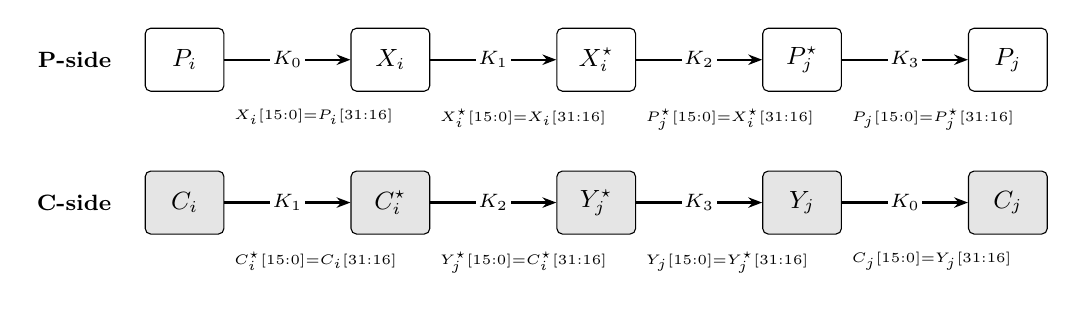
\begin{tikzpicture}[
  node distance=5mm and 16mm,
  ptn/.style={rectangle, rounded corners=2pt, draw=black, fill=white,
              minimum width=10mm, minimum height=8mm, align=center, font=\small},
  ctn/.style={rectangle, rounded corners=2pt, draw=black, fill=black!10,
              minimum width=10mm, minimum height=8mm, align=center, font=\small},
  arr/.style={-{Stealth[length=5pt]}, thick},
  klbl/.style={fill=white, font=\scriptsize, inner sep=1pt, pos=0.5},
  ptlbl/.style={font=\tiny, text=black, align=center},
  ctlbl/.style={font=\tiny, text=black, align=center},
]
 % Plaintext row
 \node[ptn] (Pi) {$P_i$};
 \node[ptn, right=of Pi] (Xi) {$X_i$};
 \node[ptn, right=of Xi] (Xsi) {$X_i^\star$};
 \node[ptn, right=of Xsi] (Psj) {$P_j^\star$};
 \node[ptn, right=of Psj] (Pj) {$P_j$};

 \draw[arr] (Pi) -- (Xi) node[klbl]{$K_0$};
 \draw[arr] (Xi) -- (Xsi) node[klbl]{$K_1$};
 \draw[arr] (Xsi) -- (Psj) node[klbl]{$K_2$};
 \draw[arr] (Psj) -- (Pj) node[klbl]{$K_3$};

 \node[ptlbl, below=1mm of Pi.south east, anchor=north west]
   {$X_i[15{:}0]{=}P_i[31{:}16]$};
 \node[ptlbl, below=1mm of Xi.south east, anchor=north west]
   {$X_i^\star[15{:}0]{=}X_i[31{:}16]$};
 \node[ptlbl, below=1mm of Xsi.south east, anchor=north west]
   {$P_j^\star[15{:}0]{=}X_i^\star[31{:}16]$};
 \node[ptlbl, below=1mm of Psj.south east, anchor=north west]
   {$P_j[15{:}0]{=}P_j^\star[31{:}16]$};

 % Ciphertext row
 \node[ctn, below=10mm of Pi] (Ci) {$C_i$};
 \node[ctn, right=of Ci] (Csi) {$C_i^\star$};
 \node[ctn, right=of Csi] (Ysj) {$Y_j^\star$};
 \node[ctn, right=of Ysj] (Yj) {$Y_j$};
 \node[ctn, right=of Yj] (Cj) {$C_j$};

 \draw[arr] (Ci) -- (Csi) node[klbl]{$K_1$};
 \draw[arr] (Csi) -- (Ysj) node[klbl]{$K_2$};
 \draw[arr] (Ysj) -- (Yj) node[klbl]{$K_3$};
 \draw[arr] (Yj) -- (Cj) node[klbl]{$K_0$};

 \node[ctlbl, below=1mm of Ci.south east, anchor=north west]
   {$C_i^\star[15{:}0]{=}C_i[31{:}16]$};
 \node[ctlbl, below=1mm of Csi.south east, anchor=north west]
   {$Y_j^\star[15{:}0]{=}C_i^\star[31{:}16]$};
 \node[ctlbl, below=1mm of Ysj.south east, anchor=north west]
   {$Y_j[15{:}0]{=}Y_j^\star[31{:}16]$};
 \node[ctlbl, below=1mm of Yj.south east, anchor=north west]
   {$C_j[15{:}0]{=}Y_j[31{:}16]$};

 % Row labels
 \node[font=\footnotesize\bfseries, text=black, left=3mm of Pi] {P-side};
 \node[font=\footnotesize\bfseries, text=black, left=3mm of Ci] {C-side};
\end{tikzpicture}}%
\caption{State layout for the baseline S/MITM attack $(16,16,16)$.
The white upper row contains plaintext-side states, and the light-gray lower row contains ciphertext-side states.
Arrows show the 16-round key chunks, and the equations below the states identify the passthrough bits.}
\label{fig:mitm-state-layout}
\end{figure}

Next, the attack guesses a 16~bit overlap value $u$.
By the passthrough property (\autoref{subsec:passthrough}), the backward peel $P_j^{\star} \xrightarrow{K_3,\,16} P_j$ fixes the \emph{high} 16~bits of $P_j^{\star}$ for free:
$P_j^{\star}[31:16] = P_j[15:0]$.
The guess $u$ supplies the unknown low half, giving the full state
\[
P_j^{\star} = P_j[15:0] \| u.
\]
Since both endpoints of the transition $(P_j^{\star},\, P_j)$ are now known, the 16~key bits $K_3$ are recovered by linear extraction (\autoref{lem:linear-step}).
The attack then computes $Y_j^{\star} = D_{16}(K_3, Y_j)$ and stores $Y_j^{\star}[15:0]$ in a hash table.

On the left side, the forward passthrough $X_i \xrightarrow{K_1,\,16} X_i^{\star}$ fixes the \emph{low} 16~bits:
$X_i^{\star}[15:0] = X_i[31:16]$.
The same overlap guess determines $X_i^{\star}[31:16] = u$.
Together $X_i^{\star} = u \| X_i[31:16]$.
The 16~key bits $K_1$ are extracted from $(X_i, X_i^{\star})$, and the attack computes $C_i^{\star} = E_{16}(K_1, C_i)$.
A hit between $C_i^{\star}[31:16]$ and $Y_j^{\star}[15:0]$ gives a candidate pair.
The attack then extracts the middle key bits $K_2$ in two independent ways, from the plaintext path and from the ciphertext path, and accepts the candidate only if both extractions agree.
Only then does the attack verify the assembled key $K = K_3 \| K_2 \| K_1 \| K_0$ against the dataset.

\subsection{General Profiles}

The optimized attack generalizes the number of peeled rounds.
Let $t_p$ be the number of rounds peeled from the plaintext side and let $t_c$ be the number of rounds peeled from the ciphertext side.
The two sides overlap in
\[
t_o = t_p + t_c - 16.
\]
The baseline attack is the special case $(t_p,t_c,t_o)=(16,16,16)$.

This generalization leads to three implementation issues.
If $t_c > t_o$, then a single overlap guess is not enough to fix the full right side state, so multiple right side candidates must be generated.
If $t_p > t_o$, then a single overlap guess is not enough to fix the full left side state, so multiple left side candidates must be generated.
The number of overlap guesses changes from $2^{16}$ in the baseline to $2^{t_o}$ in the generalized attack.

The best known-plaintext profile in~\cite{indesteege2008practical} is $(15,15,14)$.
The best chosen-plaintext profile in~\cite{indesteege2008practical} is $(20,13,17)$.
In our implementation, the generalized CPU code supports both profiles.
The current GPU code directly supports $(16,16,16)$ and $(15,15,14)$.
It also includes a GPU implementation specialized to the fixed-parameter profile $(20,13,17)$, but that GPU path does not enforce the chosen-plaintext structure that reduces the overlap loop in~\cite{indesteege2008practical}.

\paragraph{Complexity.}
The loop structure in \autoref{alg:mitm-baseline} makes the cost explicit.
For each $K_0$ and each overlap guess $u$, the attack runs one right-side pass over all records (steps $(4a)$--$(6a)$) and one left-side pass over all records (steps $(4b)$--$(6b)$).
In the baseline profile, the three outer indices $K_0$, $u$, and the record index each range over $2^{16}$ values.
Each record pass performs $t_c+t_p=32$ single-round operations of extraction and partial encryption, so one such pass costs
\[
2^{16} \cdot 2^{16} \cdot 2^{16} \cdot 32 = 2^{53}
\]
single-round operations, which is about $2^{44.0}$ full KeeLoq encryptions after dividing by $528 \approx 2^{9.0}$.
Since \autoref{alg:mitm-baseline} contains both the right-side build and the left-side probe, and then checks candidate collisions, the overall baseline cost rises to about $2^{45.0}$ full encryptions, as reported in~\cite{indesteege2008practical}.

The same reading applies to the generalized pseudocode in \autoref{app:mitm-general}.
For the generalized profile $(15,15,14)$, the overlap loop has only $2^{14}$ iterations, but each record generates $2^{t_c-t_o}=2$ right-side and $2^{t_p-t_o}=2$ left-side candidates.
This gives the standard overall estimate of about $2^{44.5}$ full encryptions.

\autoref{tab:mitm-profiles} summarizes the three parameter choices and the implementations used to evaluate them.
The baseline profile is the simplest to explain and debug.
The $(15,15,14)$ profile has a lower nominal round-operation count by a factor of about $2^{0.5}$.
As \autoref{sec:mitm-experimental} shows, the baseline profile is nevertheless faster on the measured GPU because its hash chains are shorter.
The $(20,13,17)$ profile belongs to the chosen plaintext setting.

\begin{table}[htbp]
  \centering
  \caption{S/MITM profiles and evaluation coverage.}
  \label{tab:mitm-profiles}
  \small
  \begin{tabular}{@{}lccc@{}}
    \toprule
    Profile $(t_p,t_c,t_o)$ & Data & Paper time (full encryptions) & Evaluation \\
    \midrule
    $(16,16,16)$ & $2^{16}$ KP & ${\approx}\,2^{45.0}$ & CPU, GPU \\
    $(15,15,14)$ & $2^{16}$ KP & ${\approx}\,2^{44.5}$ & CPU, GPU \\
    $(20,13,17)$ & $2^{16}$ CP & ${\approx}\,2^{44.5}$ & CPU; GPU parameters only \\
    \bottomrule
  \end{tabular}
\end{table}\nopagebreak

Here ``GPU parameters only'' means that the GPU code uses $(20,13,17)$ but not the chosen-plaintext reduction from the original attack.

\paragraph{Memory.}
For each fixed $K_0$ the implementation keeps two cache arrays of $N$ 32~bit words (the $X_i$ and $Y_i$ values) plus one hash table rebuilt for each overlap guess.
In the baseline the hash table has at most $N$ entries, so working memory is $O(N)$.
In the generalized attack each record spawns $2^{t_c - t_o}$ right side candidates, enlarging the table to $O(N \cdot 2^{t_c - t_o})$ entries.

\begin{algorithm}[htbp]
\caption{Baseline S/MITM attack (profile $16,16,16$)}\label{alg:mitm-baseline}
\SetAlgoLined
\KwIn{Dataset $\{(P_i,C_i)\}_{i=0}^{N-1}$}
\KwOut{A full 64 bit key or failure}
\For{each $K_0 \in \{0,1\}^{16}$}{
  \For{$i=0$ \KwTo $N-1$}{
    $X_i \leftarrow E_{16}(K_0,P_i)$,\quad
    $Y_i \leftarrow D_{16}(K_0,C_i)$\;
  }
  \For{each overlap guess $u \in \{0,1\}^{16}$}{
    \tcp{Right side: build hash table}
    \For{each record $j$}{
      $P_j^{\star} \leftarrow P_j[15{:}0] \| u$\;
      $K_3 \leftarrow \textsc{Extract}(P_j^{\star}, P_j, 48, 16)$\;
      $Y_j^{\star} \leftarrow D_{16}(K_3, Y_j)$\;
      $\textsc{Table.Store}(Y_j^{\star}[15{:}0],\; (Y_j^{\star}, K_3, j))$\;
    }
    \tcp{Left side: probe hash table}
    \For{each record $i$}{
      $X_i^{\star} \leftarrow u \| X_i[31{:}16]$\;
      $K_1 \leftarrow \textsc{Extract}(X_i, X_i^{\star}, 16, 16)$\;
      $C_i^{\star} \leftarrow E_{16}(K_1, C_i)$\;
      \For{each hit $(Y_j^{\star}, K_3, j)$ at key $C_i^{\star}[31{:}16]$}{
        $K_2^{(C)} \leftarrow \textsc{Extract}(C_i^{\star}, Y_j^{\star}, 32, 16)$\;
        $K_2^{(P)} \leftarrow \textsc{Extract}(X_i^{\star}, P_j^{\star}, 32, 16)$\;
        \lIf{$K_2^{(C)} \neq K_2^{(P)}$}{continue}
        $K \leftarrow K_3 \| K_2^{(C)} \| K_1 \| K_0$\;
        \lIf{$\textsc{Verify}(K)$}{\Return{$K$}}
      }
    }
  }
}
\Return failure\;
\end{algorithm}

The full generalized pseudocode is deferred to \autoref{app:mitm-general}.
In the main text, we keep only \autoref{alg:mitm-baseline}, because the generalized profile changes the overlap width and candidate multiplicities without changing the overall build-then-probe structure.

\autoref{fig:mitm-workflow} summarizes the baseline attack workflow.
For each overlap guess, the implementation first builds the right-side hash table indexed by $Y_j^{\star}[15{:}0]$ and only then probes it from the left side with $C_i^{\star}[31{:}16]$.

\begin{figure}[htbp]
\centering
\resizebox{0.92\textwidth}{!}{%
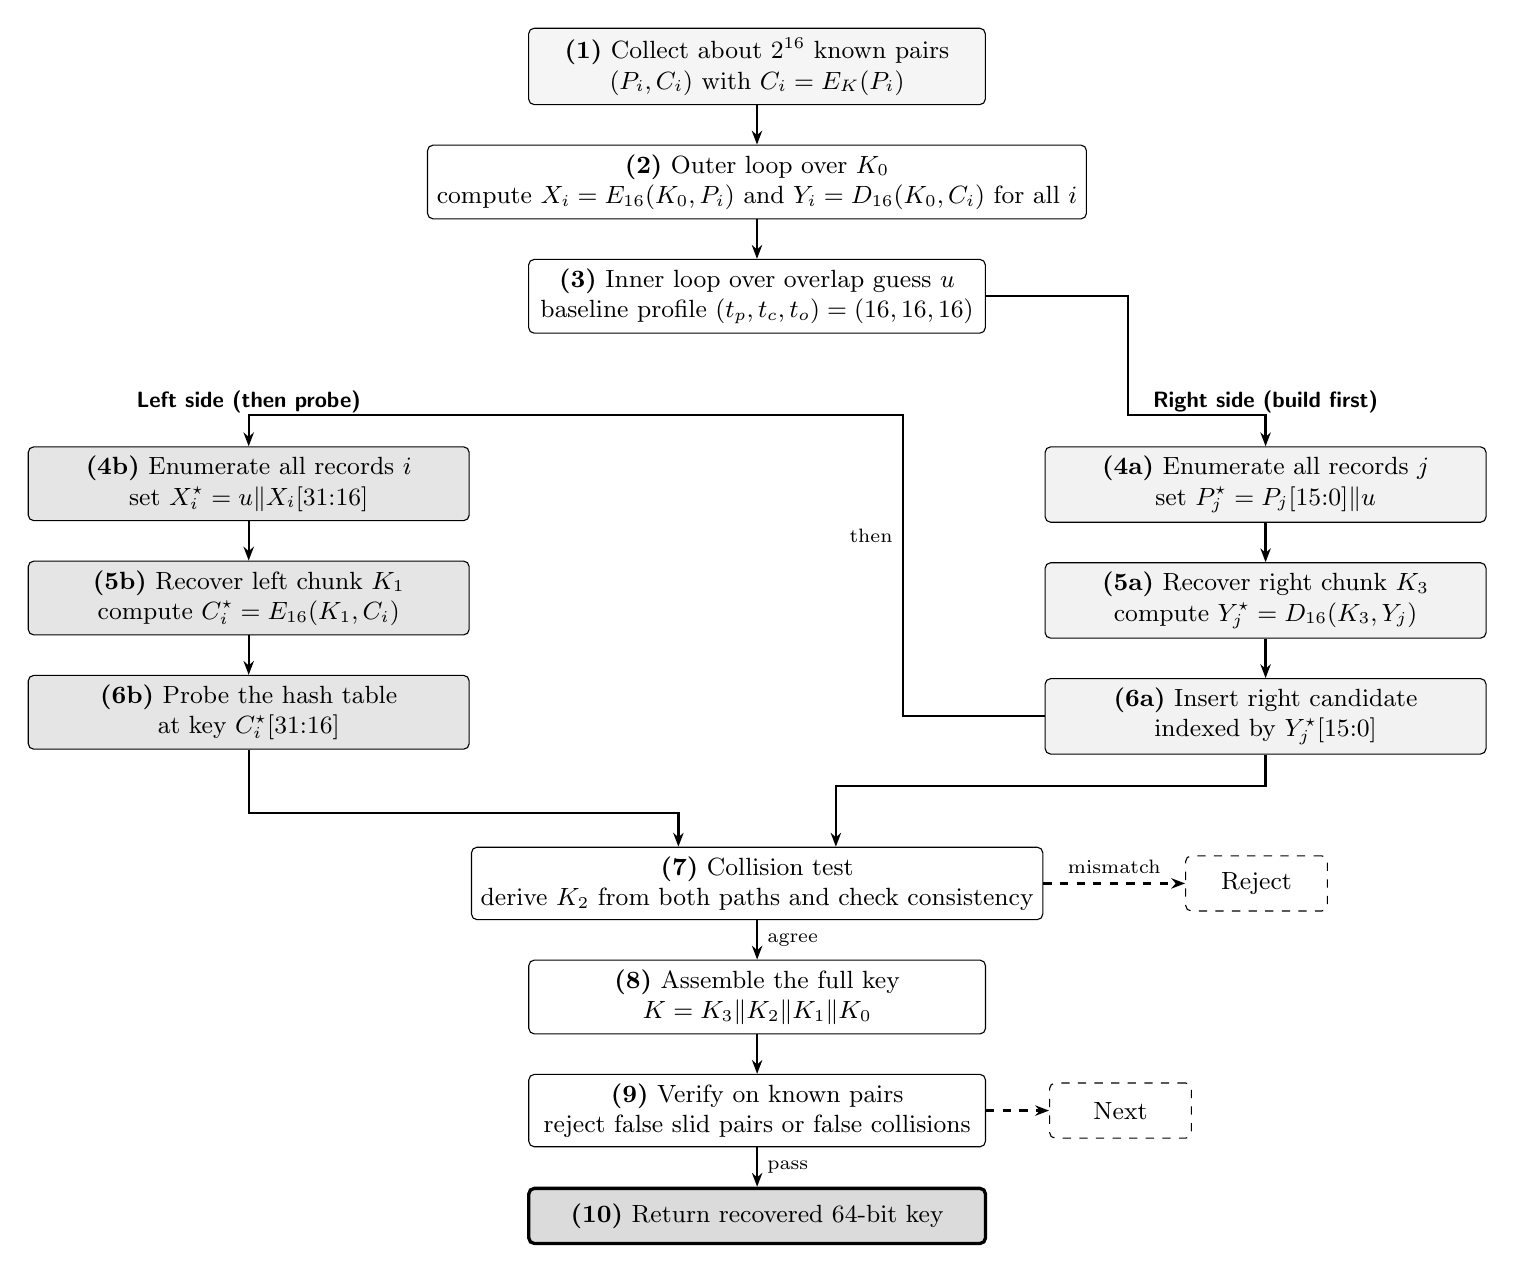
\begin{tikzpicture}[
  node distance=5mm and 5mm,
  box/.style={rectangle, rounded corners=2pt, draw=black, fill=white,
              minimum height=7mm, align=center, font=\small},
  gbox/.style={box, minimum width=5.8cm},
  rbox/.style={box, fill=black!5, minimum width=5.6cm},
  lbox/.style={box, fill=black!10, minimum width=5.6cm},
  cbox/.style={box, minimum width=5.8cm},
  obox/.style={box, fill=black!14, very thick, minimum width=5.8cm},
  dbox/.style={rectangle, rounded corners=2pt, draw=black, fill=white, dashed,
               minimum height=7mm, align=center, font=\small, minimum width=1.8cm},
  arr/.style={-{Stealth[length=5pt]}, thick},
  darr/.style={-{Stealth[length=5pt]}, thick, dashed, draw=black},
  lbl/.style={font=\footnotesize\bfseries},
]
  \node[box, fill=black!4, minimum width=5.8cm] (data) {\textbf{(1)} Collect about $2^{16}$ known pairs\\$(P_i,C_i)$ with $C_i=E_K(P_i)$};
  \node[gbox, below=of data] (k0) {\textbf{(2)} Outer loop over $K_0$\\compute $X_i=E_{16}(K_0,P_i)$ and $Y_i=D_{16}(K_0,C_i)$ for all $i$};
  \node[gbox, below=of k0] (ov) {\textbf{(3)} Inner loop over overlap guess $u$\\baseline profile $(t_p,t_c,t_o)=(16,16,16)$};

  % Two columns
  \node[lbl, text=black, below right=6mm and 20mm of ov] (rlbl) {\textsf{Right side (build first)}};
  \node[rbox, below=3mm of rlbl] (r1) {\textbf{(4a)} Enumerate all records $j$\\set $P_j^\star = P_j[15{:}0] \| u$};
  \node[rbox, below=of r1] (r2) {\textbf{(5a)} Recover right chunk $K_3$\\compute $Y_j^\star = D_{16}(K_3,Y_j)$};
  \node[rbox, below=of r2] (r3) {\textbf{(6a)} Insert right candidate\\indexed by $Y_j^\star[15{:}0]$};

  \node[lbl, text=black, below left=6mm and 20mm of ov] (llbl) {\textsf{Left side (then probe)}};
  \node[lbox, below=3mm of llbl] (l1) {\textbf{(4b)} Enumerate all records $i$\\set $X_i^\star = u \| X_i[31{:}16]$};
  \node[lbox, below=of l1] (l2) {\textbf{(5b)} Recover left chunk $K_1$\\compute $C_i^\star = E_{16}(K_1,C_i)$};
  \node[lbox, below=of l2] (l3) {\textbf{(6b)} Probe the hash table\\at key $C_i^\star[31{:}16]$};

  \coordinate (rentry) at ([yshift=4mm]r1.north);
  \coordinate (lentry) at ([yshift=4mm]l1.north);

  % Merge
  \node[cbox, below=12mm of $(r3.south)!0.5!(l3.south)$] (coll) {\textbf{(7)} Collision test\\derive $K_2$ from both paths and check consistency};
  \coordinate (rcoll) at ([yshift=4mm,xshift=-10mm]coll.north);
  \coordinate (lcoll) at ([yshift=4mm,xshift=10mm]coll.north);
  \coordinate (rcollin) at ([xshift=-10mm]coll.north);
  \coordinate (lcollin) at ([xshift=10mm]coll.north);
  \node[dbox, right=18mm of coll] (rej) {Reject};
  \node[cbox, below=of coll] (asm) {\textbf{(8)} Assemble the full key\\$K = K_3 \| K_2 \| K_1 \| K_0$};
  \node[cbox, below=of asm] (ver) {\textbf{(9)} Verify on known pairs\\reject false slid pairs or false collisions};
  \node[obox, below=of ver] (done) {\textbf{(10)} Return recovered 64-bit key};
  \node[dbox, right=8mm of ver] (fail) {Next};

  \draw[arr] (data) -- (k0);
  \draw[arr] (k0) -- (ov);
  \draw[arr] (ov.east) -- ++(18mm,0) |- (rentry) -- (r1.north);
  \draw[arr] (r1) -- (r2); \draw[arr] (r2) -- (r3);
  \draw[arr] (r3.west) -- ++(-18mm,0) |- node[pos=0.3,left,font=\scriptsize]{then} (lentry) -- (l1.north);
  \draw[arr] (l1) -- (l2); \draw[arr] (l2) -- (l3);
  \draw[arr] (r3.south) -- ++(0,-4mm) -| (lcoll) -- (lcollin);
  \draw[arr] (l3.south) -- ++(0,-8mm) -| (rcoll) -- (rcollin);
  \draw[darr] (coll) -- (rej) node[midway,above,font=\scriptsize]{mismatch};
  \draw[arr] (coll) -- (asm) node[midway,right,font=\scriptsize]{agree};
  \draw[arr] (asm) -- (ver);
  \draw[arr] (ver) -- (done) node[midway,right,font=\scriptsize]{pass};
  \draw[darr] (ver) -- (fail);
\end{tikzpicture}}%
\caption{Workflow of the baseline S/MITM attack (profile $16,16,16$).
The two light-gray shades distinguish the build and probe branches; dashed arrows denote rejected candidates.}
\label{fig:mitm-workflow}
\end{figure}

\subsection{Scope of Our Claims}

For the S/MITM attack, the asymptotic complexities are those already derived in the earlier practical S/MITM attack;
we do not claim a new asymptotic result.
Our CPU and GPU implementations realize these attack profiles directly, and we validated them on reduced and bounded instances, including deterministic tests with injected slid pairs and randomized bounded tests on modern GPUs.
The value of this part of the paper is careful explanation, exact implementation, and modern performance study.

\subsection{GPU Implementation Refinements}

The dominant probe cost is checking whether the plaintext and ciphertext paths recover the same middle key fragment.
The submitted implementation extracted both fragments completely before comparing them.
The revised GPU code derives the fragments in lockstep and stops at their first disagreeing bit.
A wrong candidate disagrees at the first bit with probability one half, so the expected comparison uses about four round operations rather than two complete fragment extractions.
This early-abort transformation is applied to all three GPU profiles and does not change the accepted candidate set.

The revised hash table stores bucket entries in contiguous ranges rather than following a linked chain.
This change reduced device memory for the $(15,15,14)$ profile from 164.5 to 140.5~MB.
Its measured speed effect was within run-to-run variation, so we claim only the memory reduction.
The generalized CPU implementation retains the original full-fragment comparison and serves as an independent correctness reference.
Consequently, CPU and GPU wall-clock values compare different implementations and should not be interpreted as a pure hardware comparison.

\subsection{Experimental Results}\label{sec:mitm-experimental}

The S/MITM attack is implemented as a generalized CPU reference and three CUDA specializations.
We tested the three GPU profiles with 18 randomized bounded recoveries at $2^8$ pairs and at most 64 low-key prefixes: 2 trials for $(16,16,16)$, 10 for $(15,15,14)$, and 6 for $(20,13,17)$.
All 18 trials recovered the expected key, and the complete regression took 32 seconds.
Per-trial wall times ranged from 0.63 to 0.69 seconds, 0.09 to 0.47 seconds, and 1.36 to 5.88 seconds for the three profiles, respectively.
These tests establish bounded implementation agreement, not full-scale success probability.

We measured full-data throughput on the platform in \autoref{subsec:gpu-platform} with $2^{16}$ known pairs and 64 low-key prefixes.
The target key lay outside the scanned range, so every run executed the complete bounded workload.
\autoref{tab:mitm-gpu-benchmark} reports the measurements and the linear extrapolation from 64 to $2^{16}$ prefixes, a factor of 1024.

\begin{table}[htbp]
  \centering
  \caption{RTX PRO~6000 S/MITM throughput.}
  \label{tab:mitm-gpu-benchmark}
  \setlength{\tabcolsep}{5pt}
  \begin{tabular}{@{}lrrrr@{}}
    \toprule
    Profile $(t_p,t_c,t_o)$ & 64-prefix time (s) & Time/prefix (s) & Full scan (h) & Memory (MB) \\
    \midrule
    $(16,16,16)$ & 17.58 & 0.275 & 5.0 & 112.5 \\
    $(15,15,14)$ & 22.37 & 0.349 & 6.4 & 140.5 \\
    $(20,13,17)$ & 130.27 & 2.036 & 37.1 & 64.5 \\
    \bottomrule
  \end{tabular}
\end{table}

The $(16,16,16)$ profile is fastest in wall-clock time despite its nominal complexity of about $2^{45.0}$ rather than $2^{44.5}$.
It stores $2^{16}$ entries in $2^{16}$ buckets, giving a mean chain length of one.
The $(15,15,14)$ profile stores $2^{17}$ entries in $2^{14}$ buckets and therefore examines about eight dependent, scattered entries per probe.
On this GPU, that memory-access cost outweighs the arithmetic saved by the narrower overlap.

A same-hardware comparison isolates the early-abort optimization: the $(15,15,14)$ 64-prefix workload decreased from 50.69 to 22.56 seconds, a factor of $2.25$.
The final 22.37-second value in \autoref{tab:mitm-gpu-benchmark} is a separate measurement of the revised code.
Conditioned on the dataset containing a slid pair and on a uniformly distributed low-key prefix, the expected hit time is about half the full-scan time.

\section{Comparison with Related Work}\label{sec:comparison}

\subsection{Fixed Point Attacks}

The FP attack in this paper should be compared first with the fixed point and cycle structure work of Courtois, Bard, and Wagner~\cite{courtois2007algebraic}.
In their work, they give two full codebook Slide Determine variants.
Version~A assumes at least one fixed point of $F$.
It succeeds for about $63\%$ of keys and costs about $2^{31}$ KeeLoq encryptions on average once the full codebook table is available.
Version~B is faster and costs about $2^{28}$ encryptions on average.
It applies to only about $30\%$ of keys because it uses a stronger condition in the filtering step.

Our FP attack is also a full codebook key recovery attack.
It targets fixed points of $F^8$ and therefore also covers cycles of $F$ with lengths $2$, $4$, and $8$.
It first recovers the low 16 key bits.
Then it recovers the remaining 48 bits exactly.
The fairest comparison is the success event.
The Courtois et al. variants succeed for about $63\%$ or $30\%$ of keys.
Our attack succeeds whenever $F^8$ has a fixed point.
Under the same random permutation heuristic, this happens with probability
$84.7\%$.
Because phase~2 is exhaustive, this is also the success probability of the current implementation.
In the 100 key benchmark, we recovered $85$ of $100$ keys, which is $85.0\%$.
This matches the model well.

Thus, in the same full codebook setting, our main advantage is higher success probability.
We do not claim a universal asymptotic runtime improvement over the Courtois et al. variants.

\subsection{Slide Based Attacks}

The slide based work on KeeLoq follows a clear path.
Bogdanov gave linear slide attacks in the full codebook setting~\cite{bogdanov2007linear}.
Aerts et al.\ later gave the practical S/MITM attack with about $2^{16}$ known plaintexts and time about $2^{44.5}$ full encryptions~\cite{indesteege2008practical}.
They also gave a chosen plaintext variant with the same paper complexity and lower CPU time in their experiments.

Our S/MITM part builds directly on that prior work.
It does not improve the paper complexity.
Instead, we explain the attack more clearly, check its logic against current code, and provide public implementations.
We should read its success probability in that lower data setting.
The familiar $\approx 63\%$ figure means that about $2^{16}$ known pairs contain at least one slid pair.
We should not compare it directly with the $84.7\%$ success probability of our FP attack, which assumes the full $2^{32}$ pair codebook.
To compare fairly, we compare attack structure and paper complexity to the 2008 paper, not wall clock times on very different hardware.
This point matters because the practical attack is easy to implement wrongly.
A small mistake in the overlap handling or bucket logic can produce wrong results without any clear sign.

\subsection{Qualitative Comparison}

The two attacks studied in this paper serve different purposes.

The FP attack uses the full plaintext space and is naturally a two-phase attack.
Its main strength is that phase~1 is fully data parallel.
Phase~2 can still recover the key even when phase~1 ranks the correct low 16 key bits poorly.
Its main weakness is the structural failure case where $F^8$ has no fixed point.

The S/MITM attack uses much less data.
Its main strength is the low data complexity of about $2^{16}$ pairs.
Its main weakness is the larger computational cost.
For this reason, we should not rank the two attacks by a single number.
They answer different questions about KeeLoq.
The FP attack studies the full codebook regime.
The S/MITM attack studies what remains possible in a much lower data regime.

\subsection{Practical Wall Clock Comparison}

For practitioners, the most relevant question is often not the asymptotic cost but the expected wall clock time on realistic hardware.
\autoref{tab:practical-runtimes} summarizes the current picture for the three attacks studied in this paper.
The BF baseline needs almost no data and works for the whole key space, but it remains slow even on a very fast GPU.
The FP attack is much faster when it applies, because phase~1 is fully data parallel and phase~2 is usually modest.
The S/MITM attack needs far less data, but its wall clock cost remains much larger.

\begin{table}[htbp]
  \centering
  \footnotesize
  \caption{Practical wall-clock comparison.}
  \label{tab:practical-runtimes}
  \setlength{\tabcolsep}{4pt}
  \renewcommand{\arraystretch}{1.05}
  \begin{tabular}{@{}>{\raggedright\arraybackslash}p{2.5cm}>{\raggedright\arraybackslash}p{2.2cm}>{\raggedright\arraybackslash}p{4.9cm}@{}}
    \toprule
    Attack & Platform & Reported result \\
    \midrule
    BF baseline &
    RTX PRO~6000 &
    Median $2^{37.36}$ keys/s; expected time 1.65 years per GPU \\
    \addlinespace
    FP attack &
    Apple M4 laptop &
    About 29 minutes for the measured benchmark \\
    \addlinespace
    FP attack &
    RTX PRO~6000 + 192-core host &
    Phase~1 below 0.05 s; mean total time 6.2 s over successful keys \\
    \addlinespace
    S/MITM $(16,16,16)$ &
    RTX PRO~6000 &
    Full scan 5.0 h; conditional expected hit time about 2.5 h (both extrapolated) \\
    \addlinespace
    S/MITM $(15,15,14)$ &
    RTX PRO~6000 &
    Full scan 6.4 h; conditional expected hit time about 3.2 h (both extrapolated) \\
    \bottomrule
  \end{tabular}
\end{table}

The BF and FP values in \autoref{tab:practical-runtimes} are direct measurements from \autoref{sec:bruteforce-experimental} and \autoref{sec:fp-experimental}.
The Apple M4 CPU line is unchanged from the original submission.
The S/MITM values come from the bounded throughput runs in \autoref{tab:mitm-gpu-benchmark} and are extrapolations, not completed full scans.

These estimates should be read with two caveats.
First, the FP attack is conditional on the presence of useful fixed points of $F^8$, which fails for about $15.3\%$ of keys under the heuristic model.
Second, the S/MITM attack times depend on scanning the low 16 key bits, so the expected time to the first hit is roughly half the full scan time for a uniformly random key.

\section{Conclusion}\label{sec:conclusion}

We studied a BF baseline and two structural attacks on KeeLoq.
The revised BF implementation reaches a median $2^{37.36}$ keys/s on an RTX PRO~6000, but one GPU still needs 1.65 years on average.
The FP attack directly refines the earlier full-codebook cycle-structure strategy by targeting fixed points of $F^8$ and using exhaustive phase~2 recovery.
Its modeled success probability is $84.7\%$, consistent with the 100-key experiment.
For the known S/MITM attack, our contribution is a clear, reproducible implementation and modern validation rather than a new asymptotic result.
Bounded GPU throughput runs extrapolate to 5.0 and 6.4 hours for the two known-plaintext profiles.
Same-hardware implementation refinements improved BF by a factor of $1.33$ and S/MITM by $2.25$.

\subsection{Future Work}

The main open question is practical black-box recovery with substantially fewer than $2^{16}$ plaintext--ciphertext pairs.
For $F=E_{64}$, $N$ pairs contain an expected $N^2/2^{32}$ slid pairs, giving success probability $1-e^{-1}$ at $N\approx2^{16}$.
At $N=2^{14}$ the expectation falls to $2^{-4}$ and the success probability to about $6.1\%$.
Beating this threshold requires a useful relation without an exact slid pair, or a way to combine weaker evidence across pairs.
Any proposal should report data, time, memory, and success probability under a realistic protocol setting.

\makeatletter
\if@anonymous\else
\subsection*{Acknowledgments}
This study was initially conducted in 2019.
Part of the accompanying source code was released in a public \href{https://github.com/hadipourh/KeeLoq}{GitHub repository} at that time, but the written analysis was not published.
In 2026, the author revisited the project, modernized and extended the codebase, added GPU implementations, and prepared the previously unpublished analysis for publication.
\fi
\makeatother

\bibliography{paper}

\clearpage

\appendix

\section{Generalized S/MITM Pseudocode}\label{app:mitm-general}

This appendix records the full generalized S/MITM pseudocode referenced in the main text.
It extends \autoref{alg:mitm-baseline} by allowing asymmetric peel lengths and by enumerating multiple left-side and right-side candidates for each overlap guess.

\begin{algorithm}[htbp]
\caption{Generalized S/MITM attack (profile $t_p,t_c,t_o$)}\label{alg:mitm-general}
\SetAlgoLined
\KwIn{Dataset $\{(P_i,C_i)\}_{i=0}^{N-1}$, profile $(t_p,t_c,t_o)$ with $t_o=t_p+t_c-16$}
\KwOut{A full 64 bit key or failure}
\For{each $K_0 \in \{0,1\}^{16}$}{
  compute $X_i$, $Y_i$ for all $i$ as above\;
  \For{each overlap guess $ov \in \{0,1\}^{t_o}$}{
    \tcp{Right side: enumerate $2^{t_c-t_o}$ candidates per record}
    \For{each record $j$}{
      \For{each $P_j^{\star}$ consistent with $ov$ and passthrough from $P_j$}{
        $K_3 \leftarrow \textsc{Extract}(P_j^{\star}, P_j, 64{-}t_c, t_c)$\;
        $Y_j^{\star} \leftarrow D_{t_c}(K_3, Y_j)$\;
        store $(P_j^{\star}, Y_j^{\star}, K_3, j)$ in hash table keyed by $Y_j^{\star}[t_o{-}1{:}0]$\;
      }
    }
    \tcp{Left side: enumerate $2^{t_p-t_o}$ candidates per record}
    \For{each record $i$}{
      \For{each $X_i^{\star}$ consistent with $ov$ and passthrough from $X_i$}{
        $K_1 \leftarrow \textsc{Extract}(X_i, X_i^{\star}, 16, t_p)$\;
        $C_i^{\star} \leftarrow E_{t_p}(K_1, C_i)$\;
        probe table at key $C_i^{\star}[31{:}32{-}t_o]$\;
        \For{each hit $(P_j^{\star}, Y_j^{\star}, K_3, j)$}{
          extract $K_\mathrm{mid}$ from both paths; continue if they disagree\;
          assemble and verify full key as in \autoref{alg:mitm-baseline}\;
        }
      }
    }
  }
}
\Return failure\;
\end{algorithm}

\section{Additional Proof Details}\label{app:proofs}

This appendix collects fuller derivations for the main mathematical claims used in the paper.
The new material does not change the attack logic; it only makes the underlying counting arguments explicit.

\subsection{Basic Facts About the Poisson Distribution}\label{app:poisson-basics}

We use the notation $X \sim \mathrm{Poi}(\lambda)$ for a Poisson random variable with mean parameter $\lambda > 0$.
Its probability mass function is
\[
\Pr[X=t] = e^{-\lambda}\frac{\lambda^t}{t!},
\qquad t=0,1,2,\dots.
\]
The two facts used most often in the paper are
\[
\mathbb{E}[X]=\lambda,
\qquad
\mathrm{Var}(X)=\lambda.
\]
We also use the zero-probability formula
\[
\Pr[X=0]=e^{-\lambda},
\]
and the tail formula
\[
\Pr[X\ge k] = 1 - e^{-\lambda}\sum_{j=0}^{k-1}\frac{\lambda^j}{j!}
= e^{-\lambda}\sum_{j=k}^{\infty}\frac{\lambda^j}{j!}.
\]
When independent Poisson variables are combined linearly, their expectation and variance are computed by the standard rules for independent random variables.
These facts are enough for all Poisson-based calculations used in the main text.

\subsection{Round-Indexed Proof of the Key-Extraction Lemma}\label{app:proof-linear-step}

Let $Y^{(0)}=A$ and $Y^{(t)}=B$ with $t \leq 32$.
Write the KeeLoq forward round as
\[
\begin{aligned}
Y^{(r+1)} &= (\varphi_r, Y^{(r)}_{31}, Y^{(r)}_{30}, \dots, Y^{(r)}_{1}), \\
\varphi_r &= \NLF(Y^{(r)}_{31},Y^{(r)}_{26},Y^{(r)}_{20},Y^{(r)}_{9},Y^{(r)}_{1}) \oplus Y^{(r)}_{16} \oplus Y^{(r)}_{0} \oplus k_r.
\end{aligned}
\]
After $t$ rounds, the feedback bit created in round $r$ appears in position $32-t+r$ of the final state $B$.
Therefore
\[
k_r = B_{32-t+r}
\oplus \NLF(Y^{(r)}_{31},Y^{(r)}_{26},Y^{(r)}_{20},Y^{(r)}_{9},Y^{(r)}_{1})
\oplus Y^{(r)}_{16} \oplus Y^{(r)}_{0},
\qquad 0 \le r < t.
\]
Because $t \le 32$, the state $Y^{(r)}$ is fully determined once the earlier key bits $k_0,\dots,k_{r-1}$ are known: start from $Y^{(0)}=A$, recover $k_0$ from $B_{32-t}$, compute $Y^{(1)}$, then recover $k_1$ from $B_{33-t}$, and so on.
Thus the $t$ key bits are recovered sequentially in $O(t)$ time, and each step yields a unique value, proving \autoref{lem:linear-step}.

\subsection{Moments of the \texorpdfstring{$F^8$}{F8} Fixed-Point Count}\label{app:proof-fp8-moments}

Under \autoref{lem:fp8-distribution}, write
\[
\mathrm{FP}_{F^8} = X_1 + 2X_2 + 4X_4 + 8X_8,
\]
where $X_d \sim \mathrm{Poi}(1/d)$ are asymptotically independent.
Using $\mathbb{E}[X_d]=\mathrm{Var}(X_d)=1/d$, we obtain
\[
\mathbb{E}[\mathrm{FP}_{F^8}] = 1\cdot 1 + 2\cdot \tfrac12 + 4\cdot \tfrac14 + 8\cdot \tfrac18 = 4.
\]
Independence gives
\[
\begin{aligned}
\mathrm{Var}(\mathrm{FP}_{F^8})
&= 1^2\mathrm{Var}(X_1)+2^2\mathrm{Var}(X_2)+4^2\mathrm{Var}(X_4)+8^2\mathrm{Var}(X_8) \\
&= 1 + 4\cdot \tfrac12 + 16\cdot \tfrac14 + 64\cdot \tfrac18 = 15.
\end{aligned}
\]
Likewise,
\[
\begin{aligned}
\Pr[\mathrm{FP}_{F^8}=0]
&= \Pr[X_1=0]\Pr[X_2=0]\Pr[X_4=0]\Pr[X_8=0] \\
&= e^{-1} e^{-1/2} e^{-1/4} e^{-1/8} = e^{-15/8}.
\end{aligned}
\]
This yields the phase~1 presence probability $1-e^{-15/8}$ used in \autoref{thm:fixedpoint-presence}.

\end{document}
